%% ----------------------------------------------------------------
%% Thesis.tex -- MAIN FILE (the one that you compile with LaTeX)
%% ---------------------------------------------------------------- 

% Set up the document
\documentclass[a4paper, 11pt, oneside]{Thesis}  % Use the "Thesis" style, based on the ECS Thesis style by Steve Gunn


% Include any extra LaTeX packages required
\usepackage[square, numbers, comma, sort&compress]{natbib}  % Use the "Natbib" style for the references in the Bibliography
\usepackage[nottoc]{tocbibind} % bind bibliography to the table of contents
\usepackage{verbatim}  % Needed for the "comment" environment to make LaTeX comments
\usepackage{vector}  % Allows "\bvec{}" and "\buvec{}" for "blackboard" style bold vectors in maths
\usepackage[table]{xcolor}
\hypersetup{urlcolor=black, colorlinks=true}  % Colours hyperlinks in black, can be distracting if there are many links and colored blue.
\usepackage{graphicx}
\graphicspath{{Figures/}}  % Location of the graphics files (set up for graphics to be in PDF format)
\usepackage{float}


%% ----------------------------------------------------------------
\begin{document}
\frontmatter      % Begin Roman style (i, ii, iii, iv...) page numbering

% Set up the Title Page
\title  {\ Automated Dockerfile Linting for Enforcing Security and Best Practices in Containerized Environments}
\authors{\ Peter Sheehan}
            
\addresses  {\groupname\\\deptname\\\univname}  % Do not change this here, instead these must be set in the "Thesis.cls" file, please look through it instead
\date       {\today}
\subject    {}
\keywords   {}

\maketitle
%% ----------------------------------------------------------------

\setstretch{1.3}  % It is better to have smaller font and larger line spacing than the other way round

% Define the page headers using the FancyHdr package and set up for one-sided printing
\fancyhead{}  % Clears all page headers and footers
\rhead{\thepage}  % Sets the right side header to show the page number
\lhead{}  % Clears the left side page header

\pagestyle{fancy}  % Finally, use the "fancy" page style to implement the FancyHdr headers

%% ----------------------------------------------------------------
% Declaration Page required for the Thesis
\Declaration{

\addtocontents{toc}{\vspace{1em}}  % Add a gap in the Contents, for aesthetics


      
This report, \thesistitle, is submitted in partial fulfillment of the requirements of \awardlevel \space in \award \space at \institutename. I, \studentname , declare that this thesis titled, \thesistitle \, and the work represents substantially the result of my own work except where explicitly indicated in the text. This report may be freely copied and distributed provided the source is explicitly acknowledged. I confirm that:

\begin{itemize} 
\item[\tiny{$\blacksquare$}] This work was done wholly or mainly while in candidature \awardlevel \space in \award \space at \institutename.
 
\item[\tiny{$\blacksquare$}] Where any part of this thesis has previously been submitted for a degree or any other qualification at \institutename \space or any other institution, this has been clearly stated.
 
\item[\tiny{$\blacksquare$}] Where I have consulted the published work of others, this is always clearly attributed.
 
\item[\tiny{$\blacksquare$}] Where I have quoted from the work of others, the source is always given. With the exception of such quotations, this project report is entirely my own work.
 
\item[\tiny{$\blacksquare$}] I have acknowledged all main sources of help.
 
\item[\tiny{$\blacksquare$}] Where the thesis is based on work done by myself jointly with others, I have made clear exactly what was done by others and what I have contributed myself.

\end{itemize}
 
 
Signed:\\
\rule[1em]{25em}{0.5pt}  % This prints a line for the signature
 
Date:\\
\rule[1em]{25em}{0.5pt}  % This prints a line to write the date
}
\clearpage  % Declaration ended, now start a new page

%%% ----------------------------------------------------------------

% The Abstract Page
\addtotoc{Abstract}  % Add the "Abstract" page entry to the Contents
\abstract{
\addtocontents{toc}{\vspace{1em}}  % Add a gap in the Contents, for aesthetics
Containerization is becoming increasingly important in software development to guarantee the security, effectiveness and manageability of containerized applications is crucial. Docker, one of the most popular container platforms relies on Dockerfiles to define the setup and configuration of containers. This means improper or inconsistent Dockerfile practices can lead to bloated,insecure, and inefficient Docker images. This project focuses on developing an automated Docker linter that enforces best practices for Docker file creation, with an emphasis on security,performance and maintainability. 

The Docker checker inspects Dockerfiles for problems like using insecure or outdated base images and having too many layers or unnecessary exposed ports as well as granting root privileges.It also. Ranks "Docker Smells" bad patterns in Dockerfile practices that lead to inefficiency and maintenance problems.The tool offers advice on which issues more urgent and important to address such, as bloated image sizes,long build processes or unnecessary dependencies to ensure a smoother container deployment. The linter recommends utilizing stage builds and optimizing base images to lessen vulnerabilities and trim down image sizes. 

The Docker linter plays a role in CI / CD pipelines by offering immediate feedback to developers to ensure consistency and enhance the quality of their Dockerised environments.This initiative automates the implementation of best practices for Dockerfiles and tackles issues such as "docker smells, this project aims to boost security and performance while making containerized applications easier to maintain and less demanding, on developers.  The new Docker checker is an expandable tool that not just identifies typical errors, in Dockerfiles but also assists companies in upholding strict compliance with their own rules and industry norms.This Docker Linter differs from other tools like Hadolint by continuously updating the best practices by using a web scraper. 
}

\clearpage  % Abstract ended, start a new page
%% ----------------------------------------------------------------

\setstretch{1.3}  % Reset the line-spacing to 1.3 for body text (if it has changed)

% The Acknowledgements page, for thanking everyone
\acknowledgements{
\addtocontents{toc}{\vspace{1em}}  % Add a gap in the Contents, for aesthetics
The acknowledgements and the people to thank go here, don't forget to include your project supervisor (term one and two)\ldots
}
\clearpage  % End of the Acknowledgements
%% ----------------------------------------------------------------

\pagestyle{fancy}  %The page style headers have been "empty" all this time, now use the "fancy" headers as defined before to bring them back


%% ----------------------------------------------------------------
\lhead{\emph{Contents}}  % Set the left side page header to "Contents"
\tableofcontents  % Write out the Table of Contents

%% ----------------------------------------------------------------
\lhead{\emph{List of Figures}}  % Set the left side page header to "List if Figures"
\listoffigures  % Write out the List of Figures

%% ----------------------------------------------------------------
\lhead{\emph{List of Tables}}  % Set the left side page header to "List of Tables"
\listoftables  % Write out the List of Tables

%% ----------------------------------------------------------------
\setstretch{1.5}  % Set the line spacing to 1.5, this makes the following tables easier to read
\clearpage  % Start a new page
\lhead{\emph{Abbreviations}}  % Set the left side page header to "Abbreviations"
\listofsymbols{ll}  % Include a list of Abbreviations (a table of two columns)
{
% \textbf{Acronym} & \textbf{W}hat (it) \textbf{S}tands \textbf{F}or \\
\textbf{LAH} & \textbf{L}ist \textbf{A}bbreviations \textbf{H}ere \\
VS & Visual Studio
\\IDE &Integrated development environment
\\npm &Node Package Manager
\\VM &Virtual Machine 
}

%% ----------------------------------------------------------------
% End of the pre-able, contents and lists of things
% Begin the Dedication page

\setstretch{1.3}  % Return the line spacing back to 1.3

\pagestyle{empty}  % Page style needs to be empty for this page
\dedicatory{For/Dedicated to/To my\ldots}

\addtocontents{toc}{\vspace{2em}}  % Add a gap in the Contents, for aesthetics

%% ----------------------------------------------------------------
\mainmatter	  % Begin normal, numeric (1,2,3...) page numbering
\pagestyle{fancy}  % Return the page headers back to the "fancy" style

%% ----------------------------------------------------------------
%% CHAPTERS
\newcounter{semester}
\setcounter{semester}{2} % change to 2 to switch to implementation phase template


\chapter{Introduction}
\label{chap:intro}
\lhead{\emph{Introduction}}
This project aims to create an automated Docker linter tool to improve the security, efficiency and maintainability of Docker images. This will be done by analysing the dockerfiles and looking for docker smells within the file.It will also force developers to follow best practices within the docker file by using preset rules.This linter helps developers with workflow and will streamline the Devops team by using the \textit{shift-left} approach. 
This tool combines two main functionalities : 
\begin{enumerate}
    \item Docker Linting for best practices:
    The Linter performs static analysis of Dockerfiles to ensure that they meet the best practices and rules.This includes detecting issues such as using outdated or large base images, running containers as root, exposing unnecessary ports, etc.
    \item Docker Smells Detection: The linter also identifies \textit{Docker Smells} - poor practices in Dockerfiles.This can cause security issues, bloating, and inefficiency. 
    By identifying these issues early on, it will lead to a more secure and smaller image. The linter will check which smells are most frequently fixed within the industry and advice the developer if it is worth fixing or not. 
\begin{figure}[ht]
  \centering
  \includegraphics[width=0.63\textwidth]{UML.png}
  \caption{High Level Overview} % Use braces {} for the caption text
  \label{fig:Overview1} % Ensure unique label
\end{figure}
\end{enumerate}

\section{Motivation}
The concept for this project initially came to mind while I was interning as a Software Security Engineer at IBM.When I was at IBM, I learned about containerisation. Specifically, he delved into Docker and Kubernetes.At the beginning of my internship, he had a discussion with a developer who had knowledge of Kubernetes and Docker images.I was taken aback when he mentioned that he needed to inspect dockerfiles to ensure they followed practices and satisfied specific security criteria.

Performing manual check of Dockerfiles to spot security vulnerabilities and inefficiencies as poor practices appeared to be a task-prone, error-prone, and time-consuming effort, particularly in extensive setups where many Docker images are deployed. It introduces complexities into the development flow but also raises the likelihood of human mistakes. Reflectively thinking back to that discussion made me recognise a need for enhancing the automation of Dockerfile assessments with a focus on ensuring security compliance and streamlining Dockerfile optimisation. 

Fascinated by this issue, I delved into exploring solutions that already existed and found out about the availability of Docker linting tools. As an example, Red Hat had created a Docker lint tool to automate some of these validations. Unfortunately, the project has been discontinued. The abandonment of such a tool in this field further emphasised the necessity for a solution that could be embraced by developers on a large scale. 

In my exploration of the topic at hand, I came across the idea of "Docker Smells," which are essentially bad practices found in Dockerfiles that can result in inefficient or insecure images that are hard to maintain.Some "Docker smells" may be insignificant or only affect the appearance of the code slightly; however, others could potentially cause performance or security problems.This discovery inspired me to create a tool that not only promotes practices but also assesses whether addressing Docker smells is necessary.This tool provides insights into which issues are crucial to resolve and which ones can be overlooked. 

By developing a Docker linter that includes these features, I intend to assist developers in managing their workload and simplifying their workflow by decreasing tasks and increasing security through issue detection.Automating these validations can enhance efficiency by reducing image size, securing configurations, and encouraging teams to adhere to practices.Teams working in high-speed environments where even small mistakes in Dockerfiles could cause problems will find this tool especially helpful.

In essence, I am driven to work on this project because I want to connect containerization with security automation and effectively create a tool that addresses the increased demand, for improved tools in the container environment space.This project reflects not my fascination with DevOps and security but also my dedication, to solving practical challenges that developers encounter in their daily tasks.  


\section{Contribution}
This project reflects a culmination of key skills and knowledge I have developed during my studies in Computer systems. The Docker linter leverages several core concepts, particularly in software development, security, and automation. Through modules like \textit{Object Orientated Programming}, \textit{Operating Systems} and \textit{Agile Processes}, I developed a deep understanding of containerisation technologies, including Docker, which forms the backbone of this project. The Linter automates the enforcement of best practices for Dockerfiles, helping developers optimise their container builds by reducing security risks, improving efficiency, and maintaining consistency.

One of the most significant contributions of this project is its focus on security. By using  modules like \textit{Network Fundamentals} and \textit{Linux Administration}, I applied best practices to ensure that the Docker linter can detect security vulnerabilities such as the use of outdated base images, running containers as root, and exposing unnecessary ports. Automating these checks helps developers adhere to  security practices earlier in their development process, aligning with the "shift-left" security philosophy that I encountered during my internship at IBM.

Furthermore, this project goes beyond standard Dockerfile linting by incorporating the analysis of \textit{Docker smells} anti-patterns that downgrade the performance and maintainability of containerised applications. My linter not only identifies these smells but also prioritises which issues are worth fixing, offering developers actionable insights to improve their Dockerfiles. This aspect of the project demonstrates both innovation and problem-solving, showcasing my ability to extend traditional solutions to meet modern software engineering needs.

In summary, this project reflects my ability to apply computer systems knowledge in a practical setting, integrating concepts such as static code analysis, DevOps practices, and security automation. It bridges academic theory with real-world application, ensuring that the skills I have acquired are used to solve meaningful problems in the area of containerised software development.

\section{Structure of This Document}
% notice how I cross referenced the chapters through using the \label tag --> LaTeX is VERY similar to HTML and other mark up languages so you should see nothing new here!
\textit{Chapter One} is a detailed introduction to the project.It gives a high overview with the aid of a diagram,discuses the motivation behind the idea, and the contribution this project may have on the industry in large. 
\textit{Chapter Two} discusses the core areas being met within computer science and determines what has been done within the industry.These areas are based on software engineering, Devops development, Cloud automation and containerisation, Docker security, and CI/CD automation. 
\textit{Chapter Three} talks about the problems within the industry that we are trying to solve as well the functional and non-functional requirements for this project.
\textit{Chapter Four} outlines the strategy for developing the Docker linter. It mentions the architecture, rick assessment,methodology and implementation plan for this project. 
\textit{Chapter Five} is the conclusion of the paper, where the project as well as any future work is discussed.  % Introduction
\chapter{Background}
\label{chap:background}
\lhead{\emph{Background}}
\section{Thematic Area within Computer Science}
This project is focused on developing a docker linter for best practices by combining multiple areas within the computer science field. 
The aim of the paper is to propose a Docker linter that enforces best practices, improving the quality of Dockerfile through the detection of Docker smells and automated refactoring suggestions. This paper has proposed a Docker Linter, which checks Dockerfiles to see whether best practices defined by the industry and best configuration practices are applied and gives recommendations to developers that can actually be acted upon. This tool will assist developers and DevOps engineers in building secure, efficient, and maintainable Docker images by automatically detecting configuration issues, ensuring consistency, and reducing human errors. Unlike other tools focused purely on vulnerability detection, this project focuses on Dockerfile optimisation and best security configuration practices at the code level.
% notice the enumerate structure to create itemized lists
\subsection{Core Topic of Project.}
    This core idea is to develop a Docker linter that parses Dockerfiles for adherence to best practices and detection of "Docker smells", which means violations of best practices and may affect Docker image security, performance, and maintainability. With the focus on optimisations at the Dockerfile level, this linter satisfies that need for a tool to improve Dockerfile quality without the use of other external services for vulnerability detection.\cite{StudyofDockerSmells}
    
\subsection{Software Engineering}
    Software Engineering is a key area in this project, focusing on maintaining and refactoring Dockerfiles without changing the external outcome.
    Software Engineering has the objective to solve industry's problems by producing good, maintainable software.\cite{softwareEng}
    The linter uses static code analysis, a software engineering technique that examines code without executing the program. This provides an understanding of the code structure and can help ensure the code adheres to the best practices. 
    
    This project aligns with software maintenance approaches since it provides continuous updates to Dockerfile best practices, ensuring that teams are always equipped with the latest rules and recommendations.Software maintenance, refers to the continuous improvement of the software artifacts\cite{canfora2001softwaremaintenance}. Docker Linter, in the context of this present project, would go a long way toward keeping teams current with the evolving best practices in Dockerfiles and hence reduces the risk of \textit{Docker Smells}, which are violations of best practices, similar to code smells \cite{DockerSmellEmpherical}. This project's automation of quality assurance ensures consistent code reviews that are less susceptible to human errors, thus adhering to principles of software engineering such as automation, consistency, and repeatability. \cite{softwareEng}
    
    It also generalises the notion of refactoring, known in software engineering as improving code or configuration files to a higher quality without changing their external behaviour. \cite{refactoring} In this case, refactoring means rewriting Dockerfiles for compliance with the best practices and avoiding Docker anti-patterns. This would allow a developer to enforce a single coding standard, thereby improving the overall collaboration within the development group and the quality of the code.
\subsection{Virtualisation}
    Virtualization is the process of creating virtual instance of a computer system.\cite{ConVSVirt} Virtualisation enhances resource efficiency and utilisation by enabling the independent operation of numerous operating systems and applications on a single physical computer by abstracting the underlying hardware. Virtual Machines (VMs) are primary products of virtualisation. A VM includes its own operating system, libraries and application files, enabling isolation between applications and underlying host systems. Each VM runs on a hypervisor which is virtual machine monitor, which means they run and monitor VMs\cite{ConVSVirt}
   
    Virtualisation has been a part of the computing scene for nearly half a century.In the 1960s and 1970s IBM developed the Control Program which led into VM/370.\cite{Virt2013} These Systems let each user run what seemed to be an isolated system, but all within a timeshared computing environment.Virtualisation has advanced dramatically over the years and is now a fundamental component in modern computing environments. The desire to maximise resource utilisation, increase system scalability, and improve isolation for security and stability have driven the development of virtualisation technologies. These earlier ideas have been expanded into enterprise-grade solutions by contemporary hypervisors like VMware ESXi, Microsoft Hyper-V, and open-source programs like KVM and Xen.\cite{Virt2013}

    The ability of virtualisation to enhance resource utilisation is one of its main contributions to this project. Multiple VMs can share physical hardware in virtualised settings, which improves resource use efficiency. By eliminating unnecessary image layers, requiring multi-stage builds, and eliminating unneeded dependencies, the Docker Linter also seeks to encourage resource-efficient Dockerfiles. This is similar to virtualization's objective of guaranteeing lean and optimised infrastructure, which is especially advantageous in cloud-native settings where resource efficiency and performance are crucial.\cite{2012virtualization}

    Despite its benefits, virtualization has limitations that highlight the value of containerization. The resource overhead of VMs, which require a full operating system, is significantly higher compared to lightweight containers that use OS-level virtualization. This project leverages the lightweight nature of containers by promoting best practices through the Docker Linter, ensuring that containerized applications remain efficient, agile, and scalable without the bulkiness of traditional VMs.\begin{figure}[ht]
  \centering
  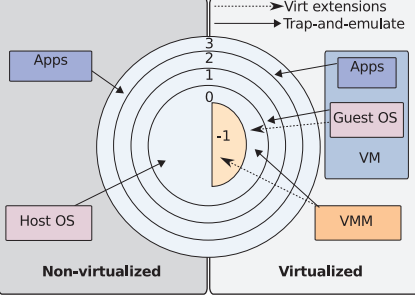
\includegraphics[width=0.63\textwidth]{Figures/Virt.png}
  \caption{overview of non-virtualized and virtualized application environments, \cite{2012virtualization}} % Use braces {} for the caption text
  \label{fig:2.2} % Ensure unique label
\end{figure}

In \ref{fig:2.2} provides a comparative overview of non-virtualised and virtualised application environments, emphasizing the abstraction and layering involved in virtualization. On the left, the non-virtualised setup demonstrates a direct relationship between applications and the host operating system, which manages the hardware resources directly. This approach is simpler but lacks isolation, making it less secure and efficient for running multiple applications concurrently.

On the right, the virtualised environment introduces additional layers of abstraction. Applications run within their own isolated virtual machines (VMs), each containing a guest operating system (OS). The hypervisor or Virtual Machine Monitor (VMM) lies beneath the VMs, providing resource allocation and ensuring the separation of environments. The hardware-level virtualisation is managed through mechanisms like trap-and-emulate or virtualization extensions, which enable the hypervisor to efficiently simulate the hardware for each VM.

This diagram highlights the key benefits of virtualisation, such as enhanced resource sharing, isolation, and flexibility, as each VM operates independently. However, it also underscores the added complexity and overhead introduced by managing virtual machines, making a compelling case for lightweight alternatives like containerisation in certain scenarios.

\subsection{Containerisation}
This project relates closely to Containerisation as Docker provides a way to deploy, maintain and run applications in the cloud. Containers have gained popularity as a lightweight alternative to virtual machines, particularly in micro services, due to their resource efficiency, scalability and flexibility. Containerisation has seen rapid growth in recent years but the one main barrier to adoption is security.\cite{sultan2019container}  In cloud environments, apps are deployed in containers, this allows for scalability as Kubernetes can automatically scale the container up or down depending on demands, better utilisation as containers use OS-level virtualisation rather than creating a separate VM, and flexibility as containers can be assigned specific CPU and memory. \cite{hardikar2021containerization}

This is important when one is performing application deployments at scale across cloud environments, and for this, the linter ensures that Docker images are optimised for performance.The linter does this by reducing unnecessary layers, enforcing multi-stage builds, and getting rid of unused dependencies, among other things, to make the Docker images minimal in size.\cite{DockerSmellEmpherical}

The Docker Linter also contributes to scalability by optimising images for horizontal scaling,where containers may be dynamically increased or decreased based on application load. The linter will aid the developer to achieve Lean, streamline images which will reduce deployment time, leading to faster response during high-load situations, it will also help decrease the attack surface, addressing docker smells and help reduce the barrier to adoption. \cite{StudyofDockerSmells}

The linter also supports operational efficiency, automating optimisation to help continuos deployment.This aligns with the goals of cloud native development, where agility, scalability and security are essential. 

This project generally aims at promoting Docker for cloud native development by offering a comprehensive way to enhance the quality of the container image, reduce cloud infrastructure costs, and ensure reliable deployments. Docker linter helps an organisation deploy more efficient, secure, and agile containers that will help to achieve a robust yet cost-effective cloud-native strategy. 

In \ref{fig:2.3} We can see the relationship between the applications, docker, the host operating system and the underlying infrastructure. At the top we can see multiple application running independently within containers which allows for isolation and efficient resource usage. 
The Docker layer sits below the applications, functioning as container runtimes that manage each container's execution environment. This setup relies on OS-level virtualisation, where containers share the same host OS kernel but remain isolated from one another, allowing resource efficiency without the need fir separate virtual machines. 
Beneath the Docker layer, The host operating systems manages the hardware by interacting with the underlying infrastructure.
This layered architecture shows the key benefits of containerisation; each application is isolated but runs on shared infrastructure, supporting scalability, flexibility and resource efficiency. 
\begin{figure}[ht]
  \centering
  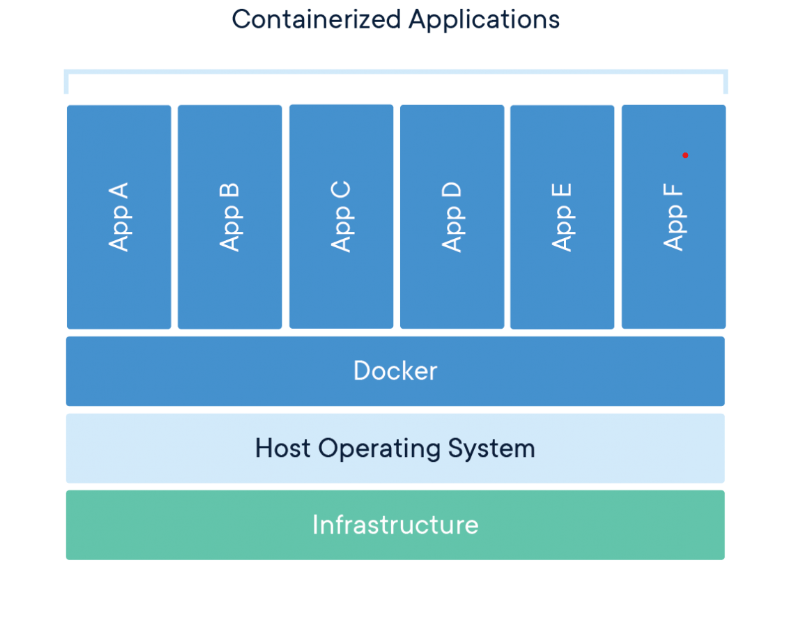
\includegraphics[width=0.73\textwidth]{Figures/container_diagram.png}
  \caption{Overview of a containerised application environment \cite{docker_cont}} % Use braces {} for the caption text
  \label{fig:2.3} % Ensure unique label
\end{figure}

\subsection{Containerisation Vs Virtualisation}
Containerisation and virtualisation are two fundamental technologies in modern computing that enable efficient utilisation of resources and application isolation, both come with several advantages and disadvantages mostly over each other.As these are both used for a wide range of application and can be used for different purposes, choosing one over the other can be of significant importance.\cite{ConVSVirt}

Virtualisation provides robust isolation and compatibility for diverse operating systems, making it a key technology in scenarios where strong security and support for legacy applications are critical.By creating fully isolated VMs, each with its own operating system, libraries and applications, virtualisation ensures that the failure of one VM does not affect others.This is important for multi-tenant environments, where security concerns are essential due to shares hardware among different users or clients.\cite{Virt2013}
However,this robust isolations comes at a cost, it introduces overhead, each VM requires substantial resources because of the need to replicate operating systems. The hypervisor, which manages these VMs add further overhead, resulting in reduced memory efficiency when compared to containerisation. 

In contrast, containerisation offers lightweight alternative that abstracts the operating system rather than the hardware. Containers share the the host OS kernel,which eliminates the need for multiple operating system instances, reducing the resource consumption.\cite{2022containerization}
This shared-kernel approach allows containers to be more agile, starting in seconds and consuming far fewer resources than VMs.\cite{Con2014docker}
However, containerisation does have limitations. While it is highly efficient, the shared-kernel model means that containers are less isolated than VMs. If the host OS is compromised, all containers running on that host are potentially at risk. In contrast, virtualisation provides stronger boundaries between applications, as each VM operates independently, with its own OS and security context. As a result, virtualisation is still highly relevant in scenarios where stronger isolation is required, such as in handling sensitive workloads or running software with strict compliance requirements.

The trade-offs between virtualization and containerization provide important context for this project. Understanding virtualization highlights the challenges that containerization overcomes, such as resource overhead and slower startup times. However, it also emphasizes the need for careful security practices in containerized environments, as containers do not provide the same level of isolation as VMs. The Docker Linter plays a crucial role in mitigating these risks by promoting best practices that reduce the attack surface, such as minimizing the number of layers, avoiding unnecessary dependencies, and enforcing the use of non-root users in containers.

\begin{figure}[ht]
  \centering
   \rotatebox{-90}{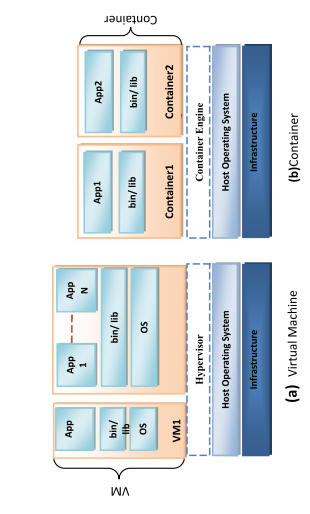
\includegraphics[width=0.63\textwidth]{Figures/Cont 143619.png}}
  \caption{fundamental differences between virtualization and containerization \cite{2022containerization}} % Use braces {} for the caption text
  \label{fig:2.4} % Ensure unique label
\end{figure}

\ref{fig:2.4} highlights the fundamental differences between virtualization and containerization, focusing on their architecture and resource utilization. Virtualization relies on hypervisors to create virtual machines (VMs), with each VM containing its own operating system, libraries, and applications. This model ensures strong isolation and compatibility for diverse workloads but comes with significant resource overhead due to the duplication of operating systems.

In contrast, containerization leverages a container engine, such as Docker, to run multiple lightweight containers that share the host operating system. Containers are more resource-efficient, as they avoid duplicating the OS, and they start quickly, making them ideal for modern cloud-native applications. The shared OS kernel and absence of hypervisor overhead allow containers to scale dynamically and deploy faster.

This distinction is crucial for the Docker Linter project, as it focuses on optimizing containerized workflows. By reducing unnecessary layers and enforcing best practices, the linter ensures containers remain efficient, scalable, and agile, aligning perfectly with the benefits of containerization depicted in the diagram.

\subsection{Docker Architecture and operational layers}
Docker's layered architecture simplifies the complicated process of application deployment and management.The figure \ref{docker_lies} shows how the programs are seperated, managed and run on the underlying hardware.

\subsubsection{Physical Sever}
At the bottom of the stack is the physical hardware, which provides the foundation for all higher layers.This includes the CPU, memory and storage necessary to run the operating system. 
\subsubsection{Operating System}
This manages the hardware and provides essential services. Docker relies on the host OS for key functionalities, such as kernel-level operations, process scheduling,etc. 
\subsubsection{Docker Engine}
The docker engine is the main layer that enables containerisation (as discussed above). The Docker Engine consists of three main components: 
\begin{itemize}
    \item \textbf{Docker Daemon:}creates, runs and manages container.
    \item \textbf{Docker CLI:}Provides the command line interface for user to interact with Docker.
    \item \textbf{Container Engine:}makes it easier to create and manage containers.\cite{schenker2020learn}
\end{itemize}
The Docker Engine allows containers to share the host OS kernel while maintaining process isolation, which reduces overhead compared to virtual machines.
\subsubsection{Comparison to Virtual Machines}
The diagram also highlights how Docker differs from traditional virtualization. Virtual machines, shown on the right, require a hypervisor to manage multiple virtualized operating systems on the same physical hardware. Each VM includes its own OS, which leads to significant overhead. In contrast, Docker containers share the host OS kernel, eliminating the need for individual OS instances and providing better performance and scalability.\cite{d}


\begin{figure}[ht]
  \centering
    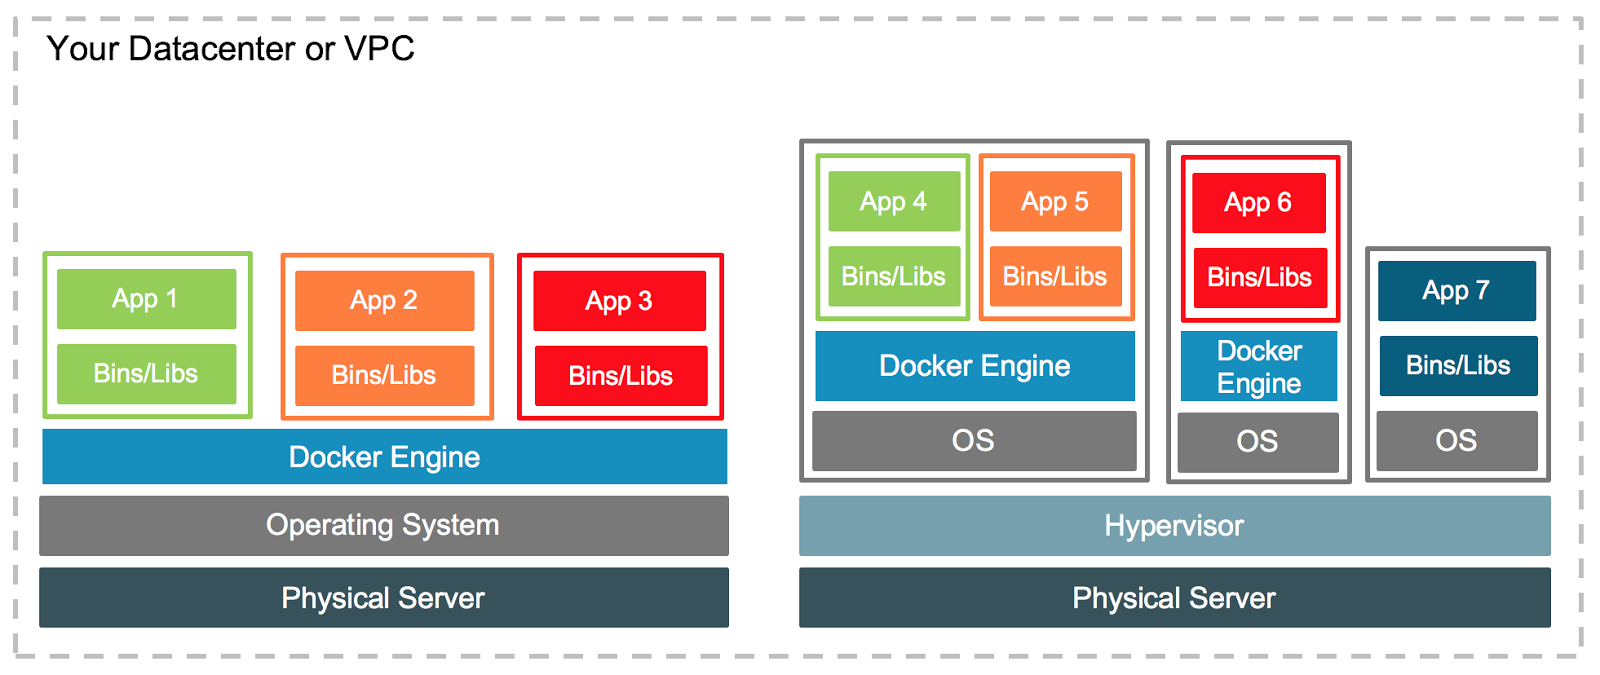
\includegraphics[width=0.93\textwidth]{Figures/difference-vm-containers.png}
  \caption{Where Docker lies \cite{docker_conttainer_where}} % Use braces {} for the caption text
  \label{docker_lies} % Ensure unique label
\end{figure}
\subsection{Docker Artifacts And Their Role}
Docker artifacts are the fundamental components generated and used throughout the Docker lifecycle.These include Dockerfiles, images, and registries, each playing a crucial role in the containerisation ecosystem. 
\begin{enumerate}
    \item \textbf{Dockerfiles:}These are the blueprint for creating Docker images. They contain the necessary instructions, such as installing the base image and copying files. A well structured Dockerfile is essential for producing an efficient, secure and scalable image.
    \item \textbf{Docker Images:}These are read only templates built from Dockerfiles.They include all the components required to run an application, such as libraries, binaries and dependencies.Images are portable and can be reused across various stages from development to production. 
    \item \textbf{Docker Registry:}A Docker registry, such as Docker Hub or private repositories, is a centralized location to store,distribute, and manage Docker images.It allows teams to share and retrieve prebuilt images for rapid deployment. \cite{DockerArtifacts}
\end{enumerate}
\subsection{Security}
 Security in this project is focused on secure configuration and best practices inside the Dockerfile itself. The linter is an application of configuration security rather than external scanning for vulnerabilities based on the detection of such risky practices as using root privilege, not specifying minimal base images, or missing secure environment configuration.
    
\textit{Shift-left} approach is the integration of continuous automated testing throughout development.
\cite{shift-left}.This will fit the concept since the security checks have been performed way in advance of the deployment. And teams can create Docker images securely. Automation of security recommendations and potential misconfiguration by Docker linter will avoid vulnerabilities with respect to Dockerfile setup. More focusing on the security through best practices rather than third-party vulnerability databases.


% Again take note of the structure, simply copy and paste this for future single figures


\section{A Review of Dockerfile quality issues and Smells}
In this section, relevant papers will be discussed in detail and how they relate to this project. Then in section 2 , similar applications will be discussed and how this project differs to them.
\subsection{Background on Docker and Its importance}
Docker is an open source tool that packages code and dependencies into a container image. It also provides an online repository for Docker images called Docker Hub.\cite{hardikar2021containerization}Unlike traditional virtual machines, which includes the OS kernel as well as the OS applications. Docker containers which are running instances of Docker Images, shares the OS kernel with the host and has it's own OS applications making it lightweight, faster and more efficient.This makes Docker a core tool in DevOps, cloud computing and containerised environments. \cite{2017Docker}

In cloud computing, Docker enables applications to be packaged and deployed,regardless of the underlying environments.Docker Desktop adds a hypervisor layer allowing the Linux applications to run on a windows or Mac OS kernel.This portability ensures that applications behave consistently across development,testing, and production stages.
In DevOps, Docker allows for continuous integration/Deployment, enabling rapid application updates, streamlined testing and seamless deployment. Containers also reduce the "it works on my machine" problem every developer faces. 

Docker's flexibility can also lead to security risks. Dockerfiles;scripts that define the instructions for building a Docker image\cite{hardikar2021containerization},play a crucial role in managing container quality and security. However without abidance to best practices, Dockerfiles can lead to containers that are bloated and hard to maintain.This veer from the best practices are called "Docker Smells". This can comprise the Docker Image security, efficiency. As companies scale their applications and rely on containers, maintaining Dockerfiles is essential to prevent vulnerabilities and security risks. Therefore, ensuring Dockerfiles adhere to best practices is essential to achieving scalable, secure and efficient images. 

\subsection{What are Dockerfile Smells?}
The concept of "Smells" comes from  software engineering where "Code Smells" are patterns in the code that indicate underlying issues or poor practices, even if they do not cause problems straight away."Docker smells" are signs of inefficient practices or configurations within Dockerfiles. These can impact a container's performance,security, or maintainability and can often lead to long-term vulnerabilities and reliability problems. 

The paper "Assessing and Improving the Quality of Docker Artifacts" \cite{DockerArtifacts} categorises these Docker smells into various types, each with it's own implications for container quality.Here are some examples of common "docker smells" and how to fix them \cite{DockerSmellEmpherical}:
\begin{enumerate}
    \item \textbf{Use of 'cd' to switch to a directory}:
    \\The WORKDIR instruction is more efficient as it sets the working directory for all subsequent instructions.It also works across build layers, making the Dockerfile more maintainable. 
    \\\textbf{FIX:} Replace \verb|RUN cd /path/to/dir| with \verb|WORKDIR /path/to/dir|. 

    \item \textbf{Missing version pinning for base image:}
    \\Having an image with the latest tag means the image will keep changing if a new version of that image is released. 
    Use specified versions. E.g Alpine. 
    \\\textbf{FIX:} Replace \verb|FROM ubuntu| with \verb|FROM ubuntu:20.04|

    \item \textbf{Missing version pinning for 'apt-get' Packages:}
    \\To ensure consistency in builds and prevent issues caused by unexpected updates in packages, pinning the version of the package ensures that image will have a stable package throughout and that any updates wont break the image or cause any security risks 
    \\\textbf{FIX:} Run \verb|apt-get install package=1.2.3| instead of \verb|Run apt-get install package|
    
    \item \textbf{Delete the apt-get lists after installing packages:}
    \\Temporary files used during package installation can bloat the image if not removed.Clearing the apt-get cache and package list after installation can reduce the image size. 
    \\\textbf{FIX:} Add \verb|RUN rm /var/lib/apt/lists/*| after \verb|apt-get install| commands.
    
    \item \textbf{Avoid Additional Packages by using '--no-install-recommends'}
    \\Using the the --no-install-recommends flag with apt-get install to prevent unnecessary packages from being installed. This Reduces the image size and minimises the potential attack surface
    \\\textbf{FIX:} Use \verb|RUN apt-get install --no-install-recommends| package. 
    
    \item \textbf{Use 'copy' instead of 'ADD' for files and Folders}
    \\Add has additional functionality (e.g extracting tar archives) that is not always needed, which can lead to unexpected behaviour.
    \\\textbf{FIX:}  Replace \verb|ADD file/path|  with \verb|COPY file/path|
    
    \item \textbf{'MAINTAINER' is deprecated:}
   \\By replacing 'MAINTAINER' with with 'LABEL', provides more flexibility and aligns with modern Docker practices.
    \\\textbf{FIX:} Replace \verb|MAINTAINER name| with \verb|LABEL maintainer='name'|
    
    \item \textbf{Set -o pipefail to avoid silencing errors in RUN instructions:}
    \\By adding \verb|SHELL ["/bin/bash","-o", "pipefail", "-c"]| to ensure errors in piped commands are not silenced.This helps in identifying errors in complex \verb|RUN|commands that use pipes.
    \\\textbf{FIX:} Add \verb|SHELL ["/bin/bash", "-o", "pipefail", "-c"]| before \verb|RUN| commands that include pipes.
    
    \item \textbf{Consolidate Multiple Consecutive RUN Instructions:}
    \\ Combining multiple \verb|RUN| instructions into a single instruction, reduces the number of layers in the Docker Image, improving build performance and reducing size.
    \\\textbf{FIX:} Replace multiple \verb|RUN| commands with one e.g 
    \begin{lstlisting}
    RUN apt-get update && \
        apt-get install -y curl wget && \
        apt-get clean && \
        rm -rf /var/lib/apt/lists/*
    \end{lstlisting}
    
    \item \textbf{Use JSON Notation for CMD and ENTRYPOINT:}
    \\Using JSON array syntax for \verb|CMD| and \verb|ENTRYPOINT|, prevents issues with shell interpretation of commands arguments, ensuring reliability. 
    \\\textbf{FIX:} Replace \verb|CMD /app/start.sh| with \verb|CMD ["app/start.sh"]|.
    
\end{enumerate}

\subsection{A literature Review of Assessing and Improving the Quality of Docker Artifacts
}
In recent years, Docker has revolutionised the way applications are developed, packaged, and deployed, becoming the backbone of cloud-native and Devops practices. Docker enables developers to create a lightweight, portable containers that encapsulates an application along with its dependencies. portability makes it easier to deploy consistently from development to diverse environments, from development to production. However, the quality of Docker artifacts, especially Dockerfiles play a crucial role in determining the overall efficiency, security and maintainability of containerised applications.

A Dockerfile serves as the blueprint for building Docker images. It's configuration determines not only the functionality of the resulting container but also, its size,build time and security.Despite its simplicity, writing optimal Dockerfiles remains a challenging task.Developers often introduce configuration flaws, known as 'Docker Smells',that compromise the effectiveness of containerisation process.These "smells" can include inefficient image layering, the use of outdated base images, and the lack of version pinning for dependencies.\cite{acharya2021docker}

The concept of "Docker Smells" draws parallels to code "smells" in traditional software development, where certain patterns indicate deeper quality issues.As identified by Giovanni Rosa, Docker smells include non-optimal practices that lead to:
\begin{enumerate}
    \item \textbf{Performance Degradation:} larger image sizes increase storage and network transfer costs, slowing down deployment pipelines.
    \item \textbf{Security Risk:} Weak configuration, such as running containers as root expose applications to potential exploits
    \item \textbf{Maintainability Challenges:} Poorly structured Dockerfiles complicate updates, leading to technical debt and slower iteration cycles. \cite{DockerArtifacts}
\end{enumerate}

The study conducted by Rosa et al, aims to assess the prevalence and impact of these "smells" across a large dataset of Dockerfiles, providing empirical evidence of their significance in real world situations.The findings reveal that these smells are prevalent and often remain unaddressed due to lack of awareness. 

"Docker smells", as explored by Rosa et al. \cite{DockerArtifacts}, are patterns of poor practices in Dockerfiles that compromise containerised application's efficiency, security and maintainability.In modern cloud native environments, the impact of these "smells" are amplified due to the scale and changeability of containers. 

\textbf{Performance Degradation} is one of the most evident consequences of Dockerfile "smells". The authors highlight that common practices, such as creating multiple layers through unoptimised \verb|RUN| commands, significantly inflate Docker image sizes. For example, each \verb|RUN| command creates a new layer in the final image, and when commands like \verb|apt-get install| are not involved in cleanup (\verb|apt-get clean|), unnecessary files are present, bloating the image. Bloated images lead to slower download times during deployment and increased storage costs, which are particularly critical in resource-constrained environments like Internet of things. \cite{securityDocker}

In terms of \textbf{security},"Dockerfile smells" introduce vulnerabilities that attackers can exploit. Running containers as root, failing to pin versions of base images, exposing unnecessary ports are practices that broaden the attack surface. Rosa et al, point out that unpinned version are particularly dangerous because they allow unintended updates to newer, potentially vulnerable versions of software components. These configurations make it harder for developers to track changes in their dependency tree, increasing the risk of deploying vulnerable containers into production environments.\cite{DockerArtifacts}

\textbf{Maintainability Issues} further worsen the challenges posed by "Docker smells". Instructions like \verb|MANTAINER|, which are deprecated still persist is older Dockerfiles and hinder automated updates.The lack of information complicates tasks such as tracking images origin, documenting build processes or applying automated refactors. Rosa et al,emphasizes that such practices obstruct collaboration, as different teams struggle to interpret poorly documented Dockerfiles, often leading to misconfiguration during updates.
In, development environments, where multiple teams manage hundreds of micro-services, these inefficiencies can add up, resulting in slower delivery cycles and higher operational costs.\cite{DockerArtifacts}

The empirical study conducted by Rose et al, stands out as one of the most comprehensive analyses of Dockerfile "smells" to date. By examining over 9 million Dockerfiles, they identified a high presence of smells, with more than 80\% of Dockerfiles containing at least one.\\The most frequently occurring smells include:
\begin{enumerate}
    \item \textbf{Missing version pinning for base images:}\\Found in a significant number of Dockerfiles, leading to unstable and potentially insecure builds.
    \item \textbf{Failure to clean package caches:}\\This results in unnecessarily large images by leaving behind temporary files causing the image to bloat. 
\end{enumerate}
These findings highlight not just the widespread nature of "Docker smells" but also their enormous impact on companies performance.On average,images with multiple "smells" were 48mb larger than optimised ones, and their build times were 20-30\% longer.These performance penalties become significant inefficiencies in large deployments, where even slight delays multiply across thousands of containers.We will dive into more detail later on in the review.

Rosa et al explored developer behaviour concerning "smell" correction.They discovered that while certain "smells" are frequently fixed especially those with immediate effect, such as missing version pinning for \verb|apt-get| packages.However, "smells" that do not have a visible impact but clearly still have inefficiencies seem to be overlooked.For example, the use of \verb|ADD| instead of \verb|COPY| is still overlooked.This suggests a knowledge gap in the industry among developers.This highlights the need for better education and more intuitive tooling.\cite{DockerArtifacts}

This study highlights the importance of automation in addressing "Docker smells". Current tools like Hadolint provide static analysis to detect these "smells", but they lack the ability to prioritise fixes based on their impact.This project aims to bridge these gaps by introducing a Docker Linter that leverages data to rank "smells" by severity, ensuring developers focus on the most critical issues first. Additionally.Further simplifying the process of maintaining high-quality Dockerfiles.

Beyond improving individual Dockerfiles, addressing "smells" has broader implications for organizational efficiency and security. In multi-cloud or hybrid cloud environments, where applications are deployed across varied infrastructure, maintaining consistent Dockerfile quality is essential. By automating the detection and resolution of "Docker smells", organizations can reduce technical debt, lower cloud infrastructure costs, and enhance the reliability and security of their applications.\cite{CI/CD2020}

As mentioned above, This study leverages a large dataset which allows the authors to systematically identify and categorise "Docker smells" and evaluate their impact on performance and security.

The dataset used in this study is one of the most extensive in the field.These Dockerfiles were collected from various sources, including public repositories on GitHub and DockerHub, to ensure a diverse sample representing real-world usage across different industries and development practices. \cite{DockerArtifacts}

The inclusion of Dockerfiles from a wide array of project, ranging from small individual efforts to large scale enterprise solutions, allowed the authors to capture a broad variety of Dockerfile quality.This dataset not only provided a robust foundation for identifying "Docker smells" but also offered insights into the common practices and the danger of Dockerfile authorship across different levels of expertise. 

To ensure the reliability of the dataset, the authors performed data cleaning and pre-processing. This involved filtering out duplicate or incomplete Dockerfiles and validating the syntax to exclude those that could not be parsed correctly, Resulting in the dataset representing a highly diverse and comprehensive sample. \cite{DockerArtifacts}

The authors employed a combination of static analysis tools and manual inspection to evaluate the Dockerfiles.
\begin{enumerate}
    \item \textbf{Use of Hadolint:} Hadolint, a lightweight linter for Dockerfiles was a key tool used. It uses predefined rules to identify "Docker smells" and flag violations of best practices. Hadolint's rules set includes checks for: 
        \begin{itemize}
            \item Using unpinned or outdated base images.
            \item Failure to clean up after package installations
            \item Use of deprecated instructions like use of \verb|ADD| instead of \verb|COPY|
        \end{itemize}
        The automated nature of Hadolint enabled the authors to rapidly analyse the large dataset, identifying millions of occurrences of Docker smells.
    \item \textbf{Manual Inspection and Trend Analysis:} While Hadolint provided a high-level overview, the authors also conducted a manual inspection to validate the findings and understand the context behind specific "smells". By examining commit histories and Dockerfile timeline,they were able to track the introduction and correction of "smells" over time. This trend analysis revealed important patterns in how developers prioritise and address "docker smells".\cite{DockerArtifacts}
    \item \textbf{Trend analysis:}The authors explored fixing trends to understand which "smells" developers tend to address most frequently and why. They examined the circumstances under which smells were introduced, the typical time frame for fixing them, and whether fixes were driven by internal policies, external pressures, or community norms.
\end{enumerate}

The research concentrated on various critical measures to assess the quality of Dockerfiles and developer behaviour. These measures offered empirical evidence into the occurrence of "Docker smells," their effects, and the success of remediation strategies.
\begin{enumerate}
    \item \textbf{Presence of "Smells":}The analysis revealed that over 80\% of the Dockerfiles contained at least one "smell", with many containing multiple "smells". The most common issues included:
    \begin{itemize}
        \item \textbf{Missing version pinning for base images:} This was among the most present "smell", without version pinning, developers risk pulling unstable or insecure versions of base images which could compromise both build reproducibility and security. 
        \item \textbf{Failure to clean the package cache:}This "smell" caused significant image bloat, as temporary files and package caches were left behind in the final image. 
        \end{itemize}
        \item \textbf{Impact on Performance and Security:} "Docker smells" were shown to have a measurable impact on both performance and security. For example:
        \begin{itemize}
            \item \textbf{Performance:} Images with multiple "smells" were, on average 48mb larger than their optimised counterparts, leading to longer download and deployment times. In environments where thousands of containers are deployed daily,these inefficiencies scale rapidly. 
            \item \textbf{Security:} Unpinned dependencies and outdated base images increased the likelihood of vulnerabilities, leaving containers exposed to potential exploits. The study highlighted specific instances where such practices had led to security breaches in production environments
        \end{itemize}
        \item \textbf{Fix Rates and Developer Adherence to Best Practices:}The study also examined developers' behaviour in addressing "Docker smells". Certain "smells", particularly those with immediate and visible impacts, such as Missing version pinning for apt-get packages, were fixed relatively frequently. In contrast, "smells" like Use COPY instead of ADD, which have less apparent consequences, were often overlooked
        \end{enumerate}
The authors noted that while awareness of "Docker smells" is growing, there remains a significant gap in understanding the long-term implications of some issues. This gap underscores the need for better education and tools to help developers prioritize and address "smells" effectively.\cite{DockerArtifacts}

The findings from Rosa et al.’s study provide a strong empirical foundation for this project. The prevalence of Docker smells and their impact on performance and security highlight the critical need for advanced tools to assist developers. While tools like Hadolint provide a good starting point, their limitations in prioritizing fixes and offering guidance leave room for improvement.

This project aims to build on these insights by developing a Docker Linter that identifies Dockerfile "smells" and ranks them based on their severity and impact. By leveraging the methods and trends identified in Rosa et al.’s study, the tool will prioritize issues to guide developers in addressing the most critical concerns. Unlike existing tools, this linter will incorporate a web scraping framework to continuously update its rules by dynamically fetching the latest best practices from trusted sources, such as Docker’s official documentation. This ensures that the tool remains relevant and up-to-date, enabling developers to maintain high-quality Dockerfiles that align with evolving standards for performance, security, and maintainability.

The current landscape of Dockerfile linting and container security tools presents a variety set of solutions, each with unique strengths and limitations. This section compares three tools: Hadolint, Snyk, and the proposed Docker Linter, focusing on their functionalities, areas of improvement, and contributions to Dockerfile and container security practices.

Hadolint is a rule-based static analysis tool specifically designed for Dockerfiles. It checks for compliance with best practices and detects Docker smells that could impact performance, security, and maintainability. One of Hadolint’s primary strengths lies in its lightweight and fast nature. It performs quick and efficient linting of Dockerfiles without requiring significant computational resources. By employing a predefined set of rules, Hadolint ensures pinned versions of base images, avoids deprecated instructions, and reduces the number of image layers. Another advantage is its seamless integration into Continuous Integration/Continuous Deployment (CI/CD) workflows, enabling teams to automate Dockerfile linting as part of their build and deployment processes. As an open-source tool, Hadolint also offers the flexibility of customization, allowing users to adapt its rules to specific project needs.\cite{wilson_2023}

\begin{figure}[ht]
  \centering
   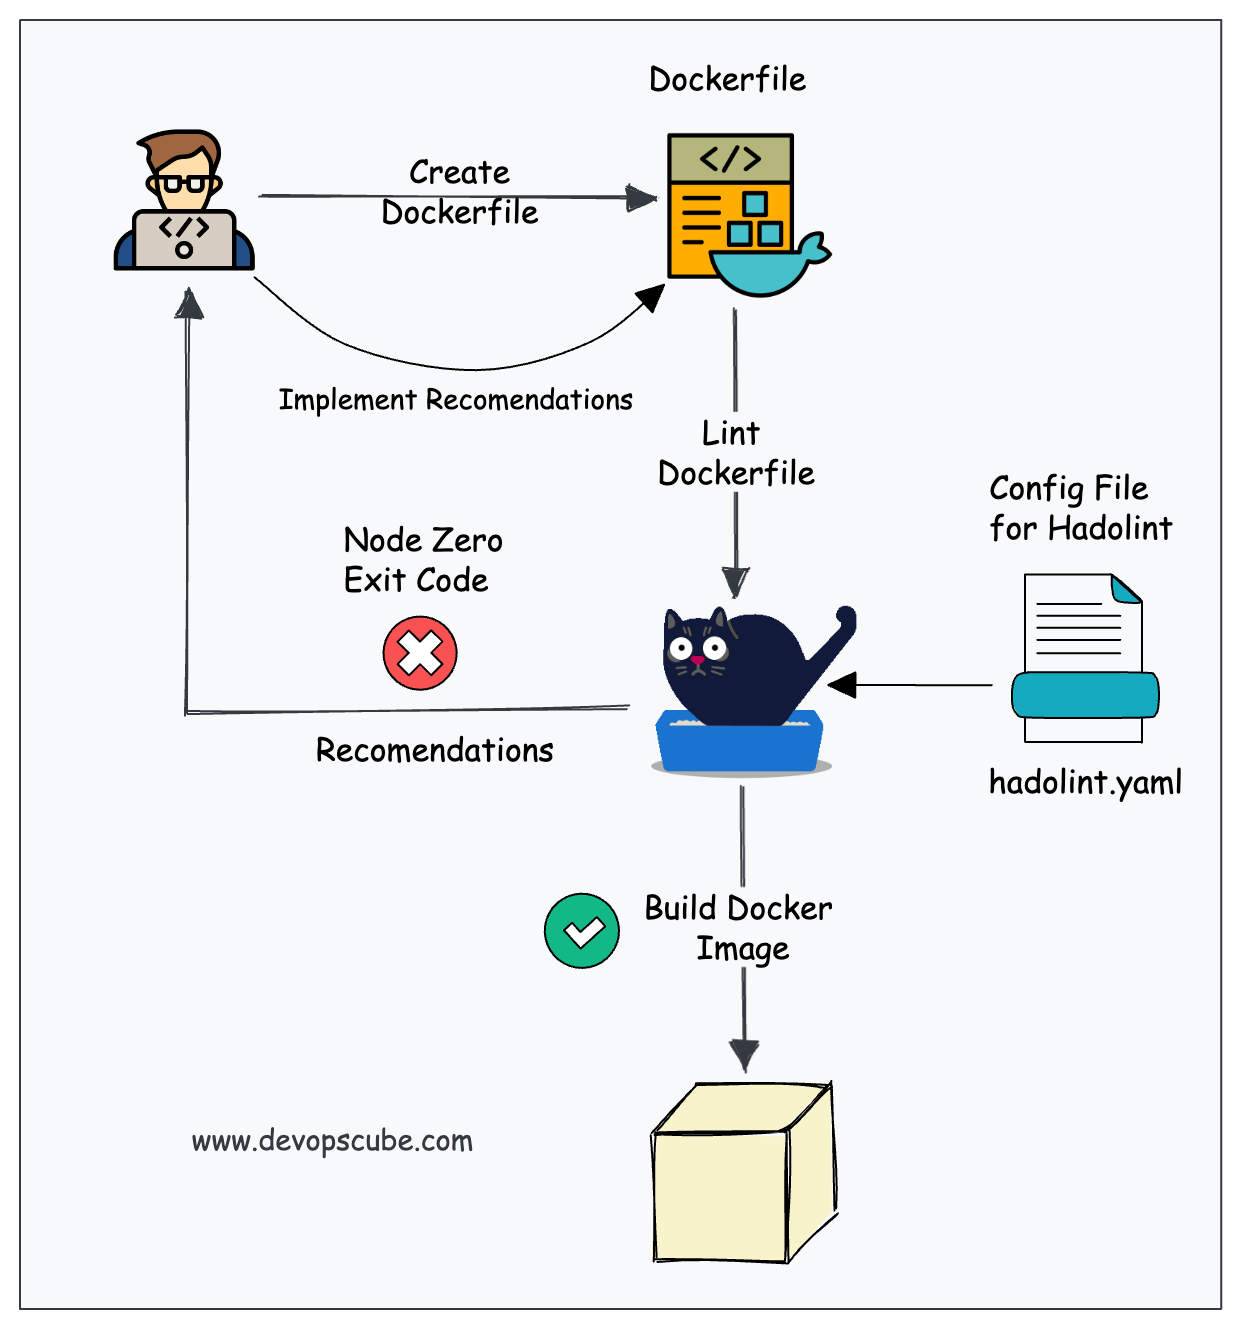
\includegraphics[width=0.58\textwidth]{Figures/hadolint-workflow.png}
  \caption{Workflow for Hadolint \cite{wilson_2023}} % Use braces {} for the caption text
  \label{fig:2.5} % Ensure unique label
\end{figure} 

Despite these advantages, Hadolint has limitations. As illustrated in Figure \ref{fig:2.5}, the workflow highlights how Hadolint integrates into the Dockerfile linting process, providing checks for syntax and best practices. However, it lacks vulnerability scanning capabilities and focuses solely on Dockerfile syntax and best practices. The tool flags issues but does not provide in-depth guidance or prioritize fixes based on their impact on performance or security, leaving developers to rely on their expertise. Moreover, Hadolint offers static feedback, providing insights only when invoked rather than real-time guidance during the development process. These limitations, while significant, provide a foundation for exploring the additional capabilities offered by other tools.

With an emphasis on both operating system packages and application dependencies, Snyk is an expert at locating and fixing vulnerabilities in container images. It can identify problems with a variety of components thanks to its extensive vulnerability database, which is updated frequently. Snyk smoothly connects with many container registries, including DockerHub and AWS ECR, and offers workable solutions, such as patching and version upgrades. Its continuous monitoring feature, which notifies users of fresh vulnerabilities in previously scanned photos even when no modifications have been made to the image itself, is a notable feature. Snyk has also improved its coverage of container security by adding the ability to check Dockerfiles for vulnerabilities.\cite{snyk_2024}
\begin{figure}[ht]
  \centering
   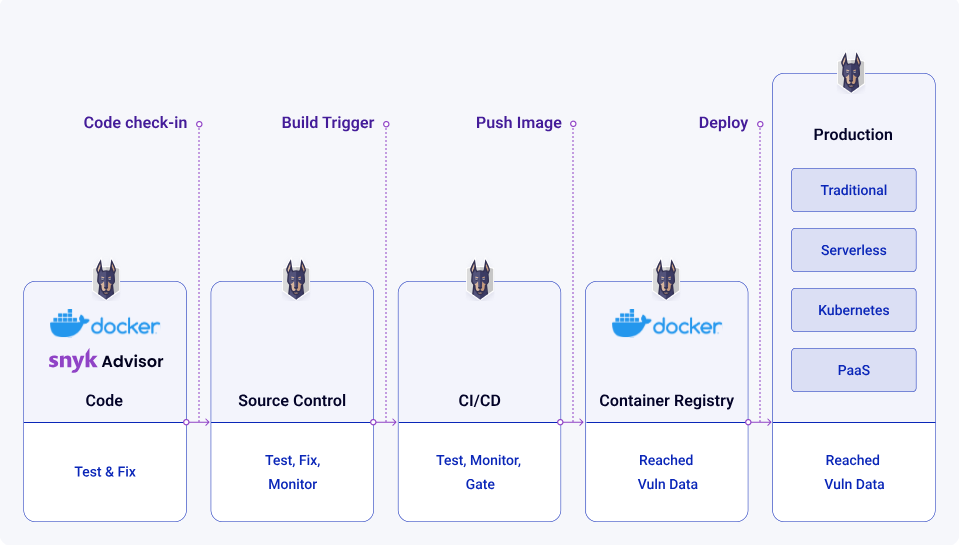
\includegraphics[width=0.9\textwidth]{Figures/snyk.png}
  \caption{Workflow for Snyk \cite{snyk2023}} % Use braces {} for the caption text
  \label{fig:2.6} % Ensure unique label
\end{figure} 

As illustrated in Figure \ref{fig:2.6}, Snyk integrates into the development workflow to provide vulnerability scanning and remediation recommendations.

But the main goal of Synk's Dockerfile scanning is to find vulnerabilities associated with base images and dependencies. It is unable to enforce recommended practices that affect performance and maintainability or identify "Docker smells". For example, Snyk doesn't examine the structure of Dockerfiles or suggest changes to reduce image size or boost build speed. Snyk does not offer comprehensive insights on compliance with best practices for Dockerfile setups, in contrast to tools such as Hadolint.\cite{snyk2023}

Synk's static rule set for Dockerfile scanning is another drawback. Although it is good at identifying known vulnerabilities, unlike the proposed Docker Linter, it does not update its rules on a regular basis to reflect changing best practices for Dockerfile optimisation. Furthermore, developers must rely on post-commit scans because Snyk does not provide real-time feedback during Dockerfile construction. This might complicate iterative development and postpone issue resolution. These shortcomings draw attention to the necessity of tools such as the Docker Linter, which place an emphasis on real-time feedback, ongoing rule modifications, and comprehensive Dockerfile analysis for efficiency and security.

The proposed Docker Linter aims to bridge gaps in existing tools by offering a specialized solution solely for Dockerfile linting and optimization. Unlike Hadolint, which provides a general static analysis of Dockerfiles, and Snyk, which primarily focuses on container image vulnerabilities, this tool focuses entirely on improving the structure and practices within Dockerfiles. By honing in on Dockerfile quality, the Docker Linter addresses inefficiencies such as unpinned base images, excessive layers, deprecated instructions, and other "Docker smells" that directly impact the performance and maintainability of resulting container images.

A unique feature of the Docker Linter is its ability to prioritise issues based on their severity and their predicted impact on performance, maintainability, and security outcomes of the built images. This prioritisation helps developers focus on critical improvements during the Dockerfile authoring process. Additionally, the linter distinguishes itself by continuously updating its rules through web scraping, ensuring adherence to the latest Docker best practices and industry standards.

Although tools such as Hadolint and Snyk are capable of delivering real-time feedback during the course of development or throughout CI/CD procedures, they depend on static or predetermined rule sets that can become outdated as time progresses. The Docker Linter, however, employs a dynamic rule update mechanism that guarantees developers have access to the most recent guidelines. This strategy, when integrated with real-time feedback provided within Integrated Development Environments (IDEs), enables developers to proactively refine Dockerfiles by addressing issues as they come up, thereby ensuring the production of high-quality container images that adhere to continuously advancing standards.

\begin{table}[ht]
    \centering
        \begin{tabular}{|p{3.5cm}|p{3.5cm}|p{3.5cm}|p{3.5cm}|}
            \hline
            \textbf{Feature} & \textbf{Hadolint} & \textbf{Snyk} & \textbf{Proposed Docker Linter} \\ \hline
            \textbf{Primary Focus} & Dockerfile linting for best practices & Vulnerability detection in container images and dependencies & Combined Dockerfile smell detection and vulnerability analysis \\ \hline
            \textbf{Smell Detection} & Yes (rule-based) & No & Yes, with dynamic rule updating \\ \hline
            \textbf{Vulnerability Scanning} & No & Yes & No \\ \hline
            \textbf{Automated Refactoring} & No & Yes & No \\ \hline
            \textbf{Continuos Rule updating} & No & No & Yes \\ \hline
            \textbf{IDE Integration} & Yes & Yes & Yes (real-time feedback) \\ \hline
            \textbf{CI/CD Integration} & Yes & Yes & Yes \\ \hline
            \textbf{Security Focus} & Limited to Dockerfile practices & Comprehensive (image and dependencies) &Limited to Dockerfile practices \\ \hline
            \textbf{Performance Optimization} & Limited to reducing image size & No & Yes (layer optimization, caching improvements) \\ \hline
            \end{tabular}
        \caption{Comparison of Hadolint, Snyk, and Proposed Docker Linter}
        \label{tab:tool_comparison}
\end{table}

The Docker Linter offers detailed explanations for each flagged issue, making it easier for developers to understand and address problems. Unlike Snyk, which focuses on image vulnerabilities, the Docker Linter emphasizes performance optimization and Dockerfile-specific analysis, ensuring that images are not only secure but also efficient and maintainable. Additionally, the tool incorporates Docker smell detection, providing developers with insights into inefficiencies at the Dockerfile level and helping them make informed decisions about prioritizing fixes.

The comprehensive capabilities of the Docker Linter are summarized in Table \ref{tab:tool_comparison}, which highlights the key features and limitations of Hadolint, Snyk, and the proposed tool. This comparison underscores the Docker Linter’s potential to serve as a comprehensive solution for improving Dockerfile quality and container security, addressing the limitations of existing tools while enhancing their strengths.

\subsubsection{Addressing Security in Docker Artifacts}
Docker containers are widely used for their efficiency and scalability, but they come with inherent security risks. The research by Rosa et al. highlights critical security issues stemming from Docker smells and proposes best practices to mitigate these risks\cite{DockerArtifacts}.This section explores the security vulnerabilities associated with Docker artifacts, examines proposed solutions in the literature, and outlines how the proposed Docker Linter can enhance security in Dockerfiles.

"Docker smells", such as running containers with root privileges, unpinned dependencies, and unnecessarily exposed ports, present significant security threats. These practices increase the attack surface, leaving containers vulnerable to exploits.\cite{Dockeranalysis}

\begin{enumerate}
    \item \textbf{Running Containers as Root:}By default,Docker containers run with root privileges, providing attackers with potential administrative access.This setup increases the likelihood of privilege escalation attacks. Privilege escalation attacks refers to a network attack aiming to gain unauthorised higher-level access within security systems.It can start with attackers exploiting vulnerabilities like running containers as root. The attackers then evaluate their access rights to gain control over sensitive information. \cite{Dockeranalysis}

    \item \textbf{Unpinned Dependencies:}The failure to pin versions of base images or software dependencies is a significant security risk in containerized environments. When a Dockerfile does not specify exact versions of the base image or installed packages, it implicitly pulls the latest available version at build time. This introduces several challenges:
    \begin{itemize}
        \item \textbf{Inconsistency in Builds:}Without version pinning, each build can result in a different image composition depending on the latest version available. This lack of reproducibility complicates debugging and quality assurance, as not all builds will be identical across different environments.For example, if a vulnerability is introduced in an newer version of a base image, containers built at different times could have different levels of security. 
        \item \textbf{Increased Vulnerability Exposure:}Unpinned dependencies make containers vulnerable to newly introduced vulnerabilities. For instance, a developer might unknowingly build a container using a base image or dependency version containing a critical security flaw, exposing the container and its host environment to potential exploits. The recent surge in supply chain attacks has further underscored the dangers of relying on unverified or automatically updated components.
        \item \textbf{Uncontrolled Updates:}Unpinned dependencies allow updates to occur automatically during builds, which might include breaking changes or introduce new bugs. These unintended changes can disrupt the application’s functionality or create unexpected security risks. Developers may find themselves scrambling to resolve issues caused by automatic updates during critical deployment phases.
        \item \textbf{Impact on Dependency Trees:}A single unpinned dependency can propagate through the dependency tree, introducing multiple layers of vulnerabilities. For example, if a base image pulls unpinned system libraries or utilities, vulnerabilities in those libraries might remain hidden until they are exploited.
    \end{itemize}
    \item \textbf{Exposed Ports and Services:}Exposing unnecessary ports in Dockerfiles can significantly increase the risk of network-based attacks. Docker containers often include services that communicate with the outside world through specific ports. If these ports are left exposed without proper justification or security measures, they become potential entry points for attackers. Here’s how this vulnerability manifests\cite{Dockeranalysis}:
    \begin{itemize}
        \item \textbf{Increased Attack Surface:} Every open port in a container represents a potential area to be exploited.Exposed ports can provide attackers with direct access to internal services or applications running within the container.This access is dangerous if the exposed service has known vulnerabilities or is misconfigured.For example, exposing admin ports without proper authentication can enable attackers to gain unauthorised control over the container.
        \item \textbf{Man in the middle attacks:}When a container communicates with external services over exposed ports, attackers can interpret this communication, particularly if it occurs over unencrypted channels. In a Man in the middle attack, the attacker positions themselves between the container and its intended recipient, capturing sensitive data such as login credentials, API keys, or private user information.Containers that expose ports for services like databases or APIs are especially vulnerable if these services lack proper encryption or authentication.

        \item \textbf{Port Scanning Exploits:}Attackers frequently use automated tools to scan for open ports on exposed containers. Once identified, these ports can be targeted for specific vulnerabilities associated with the services they host.For example, a port scan might reveal that a container is running an outdated version of a web server with known security flaws, enabling attackers to exploit these weaknesses.

    \end{itemize}
\end{enumerate}

To reduce the security risks associated with unpinned dependencies, industry best practices emphasise the importance of explicit version pinning, automated scanning, and regular updates. Developers should specify exact versions of base images and dependencies in Dockerfiles (e.g., FROM ubuntu:20.04 instead of FROM ubuntu:latest) to ensure consistent builds and minimize exposure to vulnerabilities. Automated tools like Snyk and Hadolint can help identify outdated or vulnerable dependencies, enabling timely remediation. Additionally, organisations should periodically review and update pinned dependencies to incorporate security patches and performance improvements, testing these updates in staging environments before production deployment. Together, these practices enhance container security and maintain application stability

\subsubsection{Enhancing Developer Productivity and CI/CD Pipelines}
Maintaining Dockerfiles efficiently is a significant challenge for developers, particularly in complex micro-services environments where hundreds of services must interact seamlessly. Each Dockerfile serves as a critical component for defining containerized applications, and any deviation from best practices can lead to recurring issues, including slower build times, increased resource consumption, and higher operational costs. A key hurdle is the time-intensive manual reviews that developers must perform to ensure Dockerfiles meet industry standards. These reviews often depend on individual expertise, leading to inconsistencies across projects. As a result, organizations face varied levels of compliance, increasing the likelihood of performance bottlenecks, security vulnerabilities, and unplanned downtime due to misconfigured containers

Furthermore, developers often lack visibility into the long-term consequences of "Docker smells", such as unoptimized layering, unpinned dependencies, or excessive permissions. These inefficiencies might not cause immediate failures but tend to accumulate over time, degrading system performance, bloating images, and increasing security risks. For organizations operating at scale, even minor inefficiencies in Dockerfile configurations can amplify into substantial performance penalties, particularly in cloud environments where resource optimization directly impacts costs.

The arrival of automated linting tools has revolutionized this space by offering developers a more streamlined way to enforce best practices. Tools like Hadolint analyse Dockerfiles against a predefined set of rules, automatically flagging violations such as outdated base images, excessive layers, and insecure configurations. However, these tools primarily operate in static, post-development environments, providing feedback after Dockerfiles have been written and pushed to repositories. This delayed feedback loop often leads to iterative cycles of error detection, debugging, and rework, prolonging development timelines.

The Docker Linter makes things easier for developers by giving real-time feedback right inside their coding environment, like their IDE. This means they can fix problems in their Dockerfiles as they write them. For example, if a developer uses a RUN command but forgets to clean up temporary files, the linter will immediately point it out and suggest a fix, like adding \verb|rm -rf /var/lib/apt/lists/*|. This helps keep Dockerfiles clean and efficient from the start, without waiting for later checks.

In the context of Continuous Integration and Continuous Deployment (CI/CD) pipelines, the Docker Linter plays an essential role in maintaining a high standard of quality across all deployments. CI/CD pipelines benefit greatly from automated linting as it enforces consistent best practices and prevents common errors from popping up into production. The Docker Linter integrates seamlessly into popular CI/CD tools like Jenkins, Git Lab CI, and GitHub Actions, automating the process of checking Dockerfiles for compliance at every stage of the software development lifecycle. This ensures that even in fast-paced environments where multiple teams are working on concurrent deployments, every build meets organizational quality and security standards.\cite{2022continuous}

The linter’s capabilities focus on providing developers with clear identification,prioritization of issues and providing continuous rule updates, such as redundant layers or unpinned dependencies. By highlighting the most up-to-date "smells" and ranking them based on their severity, the tool enables developers to address the most critical problems efficiently. This approach ensures that Dockerfiles are consistently optimized while maintaining a streamlined development workflow without adding unnecessary overhead..

Another significant advantage lies in the tool’s ability to streamline collaboration across distributed teams. By ensuring that all developers follow the same set of rules and receive consistent feedback, the Docker Linter reduces variability in Dockerfile quality across different projects and teams. This uniformity simplifies the debugging and troubleshooting process, as developers can rely on a common structure and set of practices for Dockerfile configurations.

Ultimately, the Docker Linter enhances developer productivity by minimizing the time and effort spent on manual reviews, reducing error rates, and ensuring that containerized applications are efficient, secure, and maintainable. It empowers organizations to achieve faster and more reliable deployments, improving the agility and scalability of their CI/CD pipelines, and reinforcing their commitment to delivering high-quality software at scale.

\subsubsection{Implications for Organizations}

The paper "Assessing and Improving the Quality of Docker Artifacts" emphasizes the critical importance of maintaining high-quality Docker artifacts for modern software development. As containerized applications continue to grow in adoption, enhancing Dockerfile and Docker image quality has become a strategic priority for organizations. Improving quality directly impacts security, cost efficiency, and operational performance, making it a cornerstone of effective container management strategies. This section explores the organizational benefits based on the findings of Rosa et al.\cite{DockerArtifacts}.

One of the most significant organizational benefits of improving Docker artifacts is enhanced security. Adhering to industry-standard best practices in Dockerfile creation helps to mitigate vulnerabilities that could arise from poor configurations. Common "Docker smells," such as unpinned dependencies or containers running with excessive privileges (e.g., root access), pose substantial risks to application security. This project addresses these issues by enabling automated detection of such smells through a linter that continuously updates its rule set via a web scraper. This ensures that the tool reflects the latest industry best practices, equipping organizations to proactively safeguard their applications against emerging threats.

Another key benefit is cost efficiency, especially in cloud environments where resource optimization directly translates to reduced expenses. Optimized Dockerfiles lead to smaller image sizes, which lower storage requirements, accelerate deployment times, and reduce network transfer costs. Rosa et al. highlight how these improvements enable organizations to achieve better resource utilization and cost savings, particularly in large-scale deployments. By focusing on eliminating unnecessary layers, enforcing multi-stage builds, and reducing redundant dependencies, the Docker Linter contributes to creating lean, high-performance images suitable for modern cloud-native strategies.

Improved Dockerfile quality also enhances development workflows by reducing the overhead associated with manual code reviews and debugging. The integration of the Docker Linter into CI/CD pipelines ensures that Docker artifacts consistently meet high-quality standards without requiring extensive manual intervention. This allows developers to concentrate on feature development rather than addressing recurring infrastructure issues. The tool's real-time feedback mechanism within IDEs further supports a streamlined development process, enabling developers to identify and fix potential issues as they write Dockerfiles, ensuring compliance with best practices from the outset.

This project's unique use of a web scraper for continuous rule updates is particularly valuable in maintaining organizational alignment with the industry's evolving best practices. Unlike other tools that rely on static rules or require manual updates, the Docker Linter ensures that developers are always working with the most up-to-date standards. This proactive approach not only enhances the relevance of the tool but also reduces the risk of technical debt associated with outdated practices.

Organizations adopting containerization strategies, particularly in hybrid and multi-cloud environments, face the challenge of ensuring consistent Dockerfile quality across diverse platforms. The Docker Linter addresses this challenge by enabling developers to produce optimized and standardized Dockerfiles, regardless of the underlying infrastructure. This ensures smoother workload migrations between cloud providers while maintaining high performance and security standards.

Additionally, the Docker Linter supports operational efficiency by helping organizations achieve faster deployment cycles and more reliable applications. By eliminating inefficiencies and enforcing best practices, the tool reduces downtime and improves application stability, allowing organizations to deliver high-quality software at scale.

The insights from Rosa et al. underscore the importance of high-quality Docker artifacts in modern software development. By adopting tools like the Docker Linter, organizations can not only enhance their container management practices but also achieve broader business goals, including cost reduction, improved security, and increased developer productivity. This project aligns closely with these objectives, providing organizations with a robust solution for maintaining consistent, high-quality Docker artifacts in a rapidly evolving industry landscape. % Background
\chapter{Problem - Enhancing Dockerfile Quality and Security through Advanced Linting}
\label{chap:problem}
\lhead{\emph{Problem Statement}}
The key question to be addressed in this chapter is: "What do I want to achieve".

This chapter outlines the problem of maintaining high-quality, secure, and efficient Dockerfiles, defines the objectives of the project, and lists the functional requirements necessary to meet these objectives.

\section{Problem Definition}
One of the key technologies in modern software development is containerization, and one of the most popular platforms for that is Docker. It allows developers to package their applications and all their dependencies into lightweight, portable containers that make it easier for them to deploy consistently across diverse environments.

Dockerfiles are at the foundation of building Docker images and therefore have a great impact on the efficiency, security, and maintainability of containerized applications. Despite their simplicity, they are often misconfigured, bringing in "Docker smells" that reduce system performance and security. Wu et al. present an empirical analysis on the occurrence of Dockerfile "smells" within 6,334 open source projects. Interestingly, they revealed that more than 84\% of the studied Dockerfiles contain at least one smell ranging from unpinned dependencies, inefficient layering practice that results in bloated images and extended build times.\cite{CharacterizingtheOccurrenceofDockerfile}\\Examples of these "smells" include:
\begin{enumerate}
    \item \textbf{Unpinned Dependencies:}\\Not locking down the exact versions of base images or software packages in Dockerfiles makes your builds unpredictable because they can pull in newer, potentially buggy, or insecure versions of software without you realizing it. Rizel et al. found this issue to be widespread in their analysis of a massive data set, highlighting how it can lead to inconsistent results and security risks, such as inadvertently using a vulnerable version of a package\cite{CharacterizingtheOccurrenceofDockerfile}.Pinning versions ensures that every time you build, you get the same reliable and secure software, minimizing surprises and vulnerabilities.
    \item \textbf{Excessive Privilege:}\\By default, Docker containers often run with root privileges,If an attacker compromises a container running as root, they can potentially take over the host system or other containers. Ksontini et al. highlighted this as a serious security flaw that can lead to privilege escalation attacks\cite{ksontini2021refactorings}.The simple fix is to Run containers with the least privilege necessary, reducing the damage an attacker can do if they get in.
    \item \textbf{Redundant Layers:}\\Every time a \verb|RUN|  instruction is used in a Dockerfile, it adds a new layer to the final image. If these instructions aren’t optimized, you end up with a bloated image, like carrying a backpack full of unnecessary items. This not only increases storage needs but also slows down deployments and consumes more bandwidth. Rizel et al. pointed out how this inefficiency can hurt performance and waste resources\cite{CharacterizingtheOccurrenceofDockerfile}.Streamlining your \verb|RUN| commands by combining them where possible helps create a leaner and faster image.
\end{enumerate}

These problems not only reduce the performance and security of individual containers but also pose significant risks to large-scale deployments. The manual effort required to identify and address "Docker smells" further worsen these issues, as manual reviews and quality checks are time-consuming and prone to human error.

While tools like Hadolint and Snyk tackle parts of the Dockerfile quality and container security puzzle, they don’t offer a complete solution. Rizel et al. note that Hadolint is great for spotting basic Dockerfile mistakes through static analysis, but it doesn’t provide detailed recommendations or real-time help as developers code\cite{CharacterizingtheOccurrenceofDockerfile}. Snyk, meanwhile, excels at finding vulnerabilities in container images and dependencies but doesn’t do much when it comes to issues specific to Dockerfiles.

This project aims to fill that gap by creating a unified tool that provides real-time feedback, detects Dockerfile issues (or "smells"), and offers clear, actionable fixes. Wu et al. emphasize that developers need tools that don’t just flag problems but also explain them and guide the user to resolve them\cite{CharacterizingtheOccurrenceofDockerfile}. By doing this, the Docker Linter aims to improve the security, efficiency, and quality of Dockerfiles, making containerized applications more reliable and easier to maintain.

Additionally, as Ksontini et al. suggest, automating fixes can help developers avoid accumulating technical debt and speed up their workflow\cite{ksontini2021refactorings}. The Docker Linter will include advanced features like automated refactoring to ensure developers spend less time fixing issues and more time building great applications.


\section{Objectives}
The primary objectives of this project revolve around creating a comprehensive solution to address the quality and security challenges inherent in Dockerfiles. Each objective is designed to fill gaps identified in existing tools and align with best practices for Dockerfile management.\\These are:
\begin{enumerate}
    \item \textbf{Automate Detection of "Docker Smells"}\\"Docker Smells" are common patterns of misconfigurations and inefficiencies that can impact a container's performance and security. This Project aims to automate the detection of these "smells",providing developers with instant feedback during development of Dockerfiles.Unlike existing static analysis tools like snyk that needs to be run manually,this Docker linter will continuously monitor the development of Dockerfiles as it can be integrated into an IDE as an extension.It will highlight "Docker smells" like unpinned dependencies, redundant layers and excessive privileges which aligns with the findings of Wu et al \cite{CharacterizingtheOccurrenceofDockerfile}, who emphasises the prevalence and impact of these "smells". 

    \item \textbf{Enhance Security in Dockerfiles}\\Security remains a critical concern in containerised environments especially since 79\% chose Docker as their container technology in 2020 \cite{CharacterizingtheOccurrenceofDockerfile}.Dockerfile often include practices that unintentionally increase the attack surface, such as running a container as root and exposing unnecessary ports.This project will check for these security vulnerability within the linting process, identifying misconfigurations and providing recommended code changes.Ksontini et al, highlights the importance of automated security checks particularly in environments where manual oversight is limited \cite{ksontini2021refactorings}.By incorporating these checks,the Docker linter will help organisations maintain a secure containerized infrastructure, reducing the likelihood of breaches and ensuring compliance with security best practices.

    \item \textbf{Optimise CI/CD Pipelines}\\As organisations move towards the adoption of DevOps and agile development approaches,the increasing popularity of containerised Continuous Integration and Continuous Deployment pipelines have become essential in software development workflow.\cite{DevSecOpsCI/CDPipeline}.Ensuring that Dockerfiles meet quality and security standards before images are built is crucial for maintaining reliable and efficient pipelines.The Project will integrate the Docker Linter within CI/CD tools like Jenkins and GitHub to ensure managers and developers can check if Dockerfiles meet the industry's best practices.By identifying and resolving Dockerfiles early in the pipeline,the Docker Linter will prevent flawed Dockerfiles from progressing into the later stages,reducing the risk of deployment failures. This aligns with the findings of Ksontini et al., who emphasize the critical role of automated quality checks in maintaining the efficiency and reliability of CI/CD workflows. 

    \item \textbf{Prioritize Issues and Generate Comprehensive Quality Reports}\\Not all Dockerfile issues carry the same level of urgency or impact. Some, like unpinned dependencies and running containers as root, represent significant security risks and should be addressed immediately, while others, such as redundant whitespace, have minimal impact on performance or security. To ensure developers focus their efforts effectively, this project will implement a severity-based ranking system. This system will prioritize issues based on their potential impact, guiding developers to address critical problems first. For instance, high-severity issues like exposed ports or unpinned dependencies will be flagged as top priorities, while less critical inefficiencies will be ranked lower.
    \\The Docker Linter will generate comprehensive quality reports for organizations. These reports will summarize key measures such as the prevalence of "Docker smells" and identified security risks(ranked by severity). .

\end{enumerate}

\section{Functional Requirements}
The following functional requirements define the key capabilities and features that the proposed Docker Linter must provide to address the challenges of Dockerfile quality and security: 
\begin{enumerate}
    \item \textbf{Real-Time Dockerfile Analysis:}\\The tool must analyse Dockerfiles in real-time as they are written, identifying common issues and providing instant feedback to developers within their ID
    \item \textbf{Smell Detection and Categorization:}\\The Docker Linter should detect and categorize "Docker smells", such as unpinned dependencies, redundant layers, and deprecated instructions, highlighting their impact on performance, security, and maintainability.
    \item \textbf{IDE Integration:}\\Seamless integration with Visual Studio Code is required to ensure that developers receive contextual recommendations directly within their workflow.
    \item \textbf{CI/CD Pipeline Compatibility:}\\The tool must integrate with CI/CD platforms like Jenkins, and GitHub Actions to enforce quality checks during automated builds and deployments.
    \item \textbf{Prioritized Issue Reporting:}\\Issues detected by the Docker Linter should be ranked based on their severity and impact, helping developers focus on resolving the most critical problems first.
    \item \textbf{Comprehensive Quality Reports:}\\The tool should generate detailed reports summarizing Dockerfile quality metrics, including the prevalence of "smells" and identified security risks. These reports should seamlessly integrate with CI/CD tools like Jenkins,and GitHub Actions providing actionable insights to help organizations monitor their Docker practices.
\end{enumerate}

\section{Non-Functional Requirements}
we now define the non-functional requirements that broadly describe how the system will operate:
\begin{enumerate}
    \item \textbf{Platform-Agnostic:}\\The Docker Linter should be platform-agnostic, working seamlessly across different operating systems and environments, including Linux, Windows and MacOS.
    \item \textbf{Performance Efficiency:}\\The linter must provide real-time feedback with minimal latency to ensure a smooth developer experience without disrupting the workflow.
    \item \textbf{Security Compliance:}\\All data handled by the tool should comply with relevant security standards, such as GDPR, to ensure user privacy and secure handling of sensitive data.
    \item \textbf{Error Reporting:}\\The tool should use standard HTTP codes to indicate operation success or failure when interacting with CI/CD pipelines or external APIs.
    \item \textbf{Continuous Monitoring:}\\The tool should support periodic or on-demand scans to track Dockerfile quality, ensuring that best practices are maintained throughout the lifecycle.
    \item \textbf{Customization and Extensibility:}\\The linter should allow users to define custom rules and extend its capabilities to accommodate specific organizational policies or unique project requirements.
\end{enumerate}

 % Problem Analysis and Design
\chapter{Implementation Approach}
\label{chap:implementation}
\lhead{\emph{Implementation Approach}}
The key question to be addressed in this chapter is: "How do I plan to achieve what I have outlined in the previous chapter".
This chapter dives into the the architecture of the Docker Linter like the framework and programming languages and how they will be used to meet the functional and non-functional requirements. 

% This chapter should comprise around 5000 words and specify your planned implementation approach. Again all sections below are suggestions and will vary significantly from project to project, the key element to be addressed is the core question of the chapter.

\section{Architecture} \label{sec:Arch}
% Describe the architecture of the solution that you have in mind, including:
The architecture is designed to ensure scalability, and ease of integration.The focus is to make sure this Linter is lightweight and can be accessed on all platforms.It combines web scraping for continuous updates on the rule database, a python based linter for rule enforcement and integration with tools like Jenkins and Visual Studio Code. 
% \begin{itemize}
%     \item Technologies involved (e.g., frameworks, programming language). 
%     \item The hardware needed to develop the project (and to support at deployment stage)
% \end{itemize}
\subsection{Technologies involved}
The following framework and technologies will be used: 
\subsubsection{Programming languages}
\begin{enumerate}
    \item \textbf{Python}\\The core linter engine and the web scraper will be written in python.Python has robust libraries for text processing and supports for web scraping.\\Key libraries used: 
    \begin{itemize}
        \item \textbf{BeautifulSoup:}For web scraping to continuously fetch updates for the rules database.
        \item \textbf{json:}For structured report generation
        \item \textbf{Flask}Create an API for interacting with the linter.
    \end{itemize}
    \item \textbf{JavaScript}\\This will be used to develop the visual studio extension, as VS gives you an option between typescript and JavaScript.
\end{enumerate}
\subsubsection{Web Scraping Framework}
Web scraping refers to the automatic extraction procedure of data from websites using software. It allows us to extract data from text such as HTML, Which allows continuous updates to Dockerfile best practices are critical to ensure that the linter remains relevant.
BeautifulSoup and Requests will be the primarily used frameworks used for the web scraping.\cite{webscraping}
Web scraping involves the creation and integration of two software programs: A crawler and a scraper.
The crawler downloads data from the internet, then the scraper extracts important information in its raw form from the downloaded data and stores it in a database. \cite{webscraping}

\textbf{BeautifulSoup:}
\begin{itemize}
    \item This is a python library that allows the user to retrieve structured data from a webpage. It can be used for parsing HTML and XML, furthermore, it is much easier to use when comparing it to regular expression( a Python package) since it has fewer steps for navigating and examining a parse tree. Compared to the other tools like Regular expression or Lxml, BeautifulSoup is the slower option but suits perfectly for the linter needs a limited amount of rules. 
    \item It has the ability to automatically convert out coming document into UTF-8 and incoming document into Unicode, so the user does not need to keep track of encodings unless the document does not specify one. \cite{webscraping}
\end{itemize}
\textbf{Requests:}
\\Requests is a Python library that is used to send HTTP requests to retrieve data from the Web.It is a powerful yet easy-to-use tool that simplifies interactions with web servers, making it ideal for integration into the web scraping framework. \cite{pypy_2024}
\begin{itemize}
    \item Requests lets developers concentrate on data extraction and processing by abstracting away the hassles of sending HTTP requests, like managing sessions, cookies and headers. 
    \item Offers flexibility in communicating with different websites by supporting all major HTTP methods, like GET,POST,PUT,etc. 
    \item Provides robust and dependable web scraping by automatically addressing typical HTTP challenges like timeouts and status code failures. The lightweight performance of the linter is maintained by its efficient and lightweight design, which guarantees low latency when retrieving web pages. 
    \item Easily integrates with BeautifulSoup to parse the retrieved HTML data, resulting in a unified process for obtaining best practices. 
\end{itemize}

When collecting data from reliable sources such as, Docker's official documentation, SSL support is essential because it guarantees secure connection by supporting HTTPS right out of the box.

\textbf{Integrated Process:}
\\Requests and BeautifulSoup work together to offer a simplified method of web scrapping. 
\begin{itemize}
    \item Fetching web pages: To retrieve HTML content from dependable sources, HTTP GET requests are sent using requests. 
    \item Data Extraction and Parsing: BeautifulSoup extracts the relevant data like Docker Best Practices after parsing the HTML text. 
    \item Database storing: To keep the linter current without being dependent on a web connection, the extracted rules are processed and then saved in a local SQlite database for offline use. 
\end{itemize}

\subsubsection{Visual Studio Extension Development}
The VS Code API and a mix of web-based and IDE's specific tools are used in the development of a Visual Studio Code plugin/extension for Dockerfile linting.\\For developers, this revised method guarantees a productive, immersive and easy to use experience.\\List of tools that will be used: \\
\textbf{JavaScript:}
\begin{itemize}
    \item JavaScript is the foundation for creating VS code extensions. It is flexible and supported by a wide variety of modules accessible through npm and will be primarily used for scripting within the browsers. 
    \item It will be used for the core functionalities such as triggering linting commands and displaying results within the VS code environment. 
\end{itemize}
\textbf{Node.js:}
\\Node.js extends JavaScript's capabilities to run outside a browser environment. 
It provides access to system level features and APIs that JavaScript, in a browser, cannot access. 
\begin{itemize}
    \item \textbf{File System Access:} Reading and writing files like Dockerfiles directly from the disk. 
    \item \textbf{Process Management:}Running external programs like docker linters using modules like child process.
    \item \textbf{VS code extensions run in Node.js:} As VS code is built on Electron, which uses Node.js , extensions for VS code run in a Node.js runtime allowing developers to utilise the system level APIs
\end{itemize}

\textbf{Node Package Manager (npm):}
\\npm simplifies dependency management, ensuring extensions have access to the latest libraries and tools. 
\begin{itemize}
    \item Manages packages like Axios and XML parsers. 
    \item Streamlines the installation and updating of dependencies required for the extension's development and functionality. 
\end{itemize}

\textbf{VS Code API:}
\begin{itemize}
    \item The API provides direct access to VS Code's editor, allowing developers to  customise the UI. 
    \item Used to help Display issues in the Problems panel and highlights them directly in the Dockerfile editor.
\end{itemize} 

\textbf{Yeoman Generator:}
\begin{itemize}
    \item Yeoman scaffolds new VS Code extension projects with boilerplate code and a well-structured file system, reducing setup time.
    \item Provides a pre-configured project structure that includes necessary files like package.json, extension.js, and configuration settings.
    \end{itemize}

\subsubsection{CI/CD Integration: Jenkins}
Integration with Jenkins ensures the Docker Linter is part of the automated build and deployment pipeline.This guarantees that Dockerfiles meet quality standards before reaching production. 
\begin{itemize}
    \item Automates linter execution during build stages.
    \item Allows flexible scripting of quality checks.
\end{itemize}
Workflow: 
\begin{itemize}
    \item Dockerfiles are linted during the "Linting" stage of the pipeline.
    \item Reports are generated and archived for review.
    \item Builds fail if critical issues are detected, enforcing quality gates.
\end{itemize}

\subsection{Database : SQLite}
SQLite is chosen over MySQL for this Docker Linter Project due to its simplicity and lightweight nature.\cite{SQLite}As this project will not have multiple user access and does not needs robust security and authentication features. SQLite appears to be the better option for this project. \cite{mysql}
\\Key Functions:
\begin{itemize}
    \item Stores best practices fetched via web scraping
    \item Ensures the linter operates offline with the most recent rules.
\end{itemize}
Tables:
\begin{itemize}
    \item Columns: Rule ID, Description, Severity, Last Updated.
    \item Purpose: Stores dynamically updated best practices.
\end{itemize}
\subsubsection{Version Control: GitHub}
GitHub will host the project code, enabling collaboration and continuous integration
Key Features: 
\begin{itemize}
    \item Automates testing of the linter for quality assurance.
    \item Ensures code changes do not break existing functionality.
    \item Allows contributors to suggest enhancements and submit pull requests. %LOOK BACK OVER THIS 
    \item Tracks issues and feature requests through GitHub's Issue Tracker.
\end{itemize}

% Provide a high level view of the system you have in mind, including any package of classes, what is it responsible for and what other packages it communicates to. Provide a high level view of the database (or structure) needed to support the project, including what each table/document is responsible for and the hierarchy among them. You need to be as specific here as you can, why? Because this will aid you in identifying parts of the project you are vague on, 
% this may be fine for some components but cause problems in term 2 for others. If you have hardware element in your project this is also where you provide a high level view of how these elements integrate into the project. So for a project that is cyber-physical you will have both a hardware and software architectural diagram. N.B. This is NOT a full system design but a high level overview of what you can credibly develop. This architecture should be informed by prototyping activity. 

% Some of the implementation focused projects may describe how do you envision tackling the functional requirements of your project via a set of use-cases. DFDs are also helpful here to understand elements of your project that may cause problems. You should describe the role of the different parts of the architecture of the solution, and the interaction among them.



\section{Risk Assessment}


% Identify any potential risk precluding you from successfully complete your project. This section is really important and often neglected by students resulting in fatal risks occurring in some projects. Make sure to give this section the time it requires. Classify the risk according to their importance, possibility of arising and enumerate the decisions you can make to anticipate them or mitigate them (in case they finally arise). Table \ref{tab:ProjRisks} may help with this classification. This section should include your mitigation approach for any critical risks.

\begin{table}[h]
\centering
\scriptsize
\caption{Initial Risk Matrix for the Docker Linter Project}
\begin{tabular}{|p{2cm}|p{2cm}|p{2cm}| p{2cm} |p{2cm}| p{2cm}|}
\hline \bf Frequency/ Consequence & \bf 1-Rare & \bf 2-Remote & \bf 3-Occasional & \bf 4-Probable & \bf 5-Frequent \\ [10pt]

\hline \bf 4-Fatal & \cellcolor{yellow!50} Issues with integrating CI/CD tools like Jenkins & \cellcolor{red!50} Data loss during database updates & \cellcolor{red!50} Major bug in rule-checking algorithm & \cellcolor{red!50} Failure to meet unique feature requirements & \cellcolor{red!50} \\ [10pt]

\hline \bf 3-Critical & \cellcolor{green!50} Outdated scraped rules & \cellcolor{yellow!50}  & \cellcolor{yellow!50} Rule conflicts across sources & \cellcolor{red!50} Poor performance with large Dockerfiles & \cellcolor{red!50} Web scraper failure \\ [10pt]

\hline \bf 2-Major & \cellcolor{green!50}  & \cellcolor{green!50}  & \cellcolor{yellow!50} Missing some smells during analysis & \cellcolor{yellow!50}  & \cellcolor{red!50}  \\ [10pt]

\hline \bf 1-Minor & \cellcolor{green!50} & \cellcolor{green!50} Rare formatting issues in reports & \cellcolor{green!50}  & \cellcolor{yellow!50}  & \cellcolor{yellow!50}  \\ [10pt]
\hline
\end{tabular} \\
\label{tab:ProjRisks}
\end{table}

\subsection{Detailed Risk Assessment}
\textbf{Risk 1: Issues with Integrating CI/CD Tools Like Jenkins}
\begin{itemize}
    \item \textbf{Frequency:}Rare 
    \item \textbf{Consequences:}Fatal 
    \item \textbf{Mitigation:}Rigorous testing with Jenkins pipelines during development and creating clear integration                       documentation to ensure seamless compatibility. 
\end{itemize}
\textbf{Risk 2: Data Loss During Database Updates }
\begin{itemize}
    \item \textbf{Frequency:}Remote 
    \item \textbf{Consequences:}Fatal 
    \item \textbf{Mitigation:}Rigorous testing with Jenkins pipelines during development and creating clear integration documentation to ensure seamless compatibility. 
\end{itemize}
\textbf{Risk 3: Major Bug in the Rule Checking Algorithm }
\begin{itemize}
    \item \textbf{Frequency:}Occasional 
    \item \textbf{Consequences:}Fatal 
    \item \textbf{Mitigation:}Ensure regular unit testing and peer reviews are being implemented.
\end{itemize}
\textbf{Risk 4: Failure to Meet Unique Feature Requirements }
\begin{itemize}
    \item \textbf{Frequency:}Probable
    \item \textbf{Consequences:}Fatal 
    \item \textbf{Mitigation:}Guarantee delivery of unique features by setting a clear deadline and test the web scraper continuously. 
\end{itemize}
\textbf{Risk 5: Outdated Scraped Rules }
\begin{itemize}
    \item \textbf{Frequency:}Rare 
    \item \textbf{Consequences:}Critical 
    \item \textbf{Mitigation:}Schedule regular scraper runs and implement notifications for failures in scraping processes. 
\end{itemize}
\textbf{Risk 6:Rule Conflicts Across Sources }
\begin{itemize}
    \item \textbf{Frequency:}Occasional 
    \item \textbf{Consequences:}Critical 
    \item \textbf{Mitigation:}Add a manual validation step to ensure that rules from trusted sources align and avoid inconsistencies.
\end{itemize}
\textbf{Risk 9: Poor Performance with Large Dockerfiles}
\begin{itemize}
    \item \textbf{Frequency:}Probable
    \item \textbf{Consequences:}Critical 
    \item \textbf{Mitigation:}Optimize the rule-checking algorithm and implement caching mechanisms to improve performance.
\end{itemize}
\textbf{Risk 10: Web Scraper Failure}
\begin{itemize}
    \item \textbf{Frequency:}Frequent
    \item \textbf{Consequences:}Critical 
    \item \textbf{Mitigation:} Build robust error-handling mechanisms and regularly update the scraper to adapt to structural changes in source websites.
\end{itemize}
\textbf{Risk 11: Minor Misalignments in IDE Integration}
\begin{itemize}
    \item \textbf{Frequency:}Rare
    \item \textbf{Consequences:}Rare
    \item \textbf{Mitigation:} Conduct rigorous testing of IDE functionality and gather user feedback to resolve discrepancies.
\end{itemize}
\textbf{Risk 12: Occasional Linter Feedback Delays}
\begin{itemize}
    \item \textbf{Frequency:}Remote
    \item \textbf{Consequences:}Major
    \item \textbf{Mitigation:} Optimize the linter’s performance, particularly for real-time feedback in IDEs and CI/CD integrations.
\end{itemize}
\textbf{Risk 13: Missing Some Smells During Analysis}
\begin{itemize}
    \item \textbf{Frequency:}Occasional
    \item \textbf{Consequences:}Major
    \item \textbf{Mitigation:} Enhance the rule-checking algorithm and ensure comprehensive coverage of all relevant Docker smells.
\end{itemize}
\textbf{Risk 14: Rare Formatting Issues in Reports}
\begin{itemize}
    \item \textbf{Frequency:}Remote
    \item \textbf{Consequences:}Minor
    \item \textbf{Mitigation:} Implement robust formatting checks in the reporting module to ensure consistency.
\end{itemize}

\section{Methodology}
% Describe your personal approach on how to tackle the different parts of this project, including:
% \begin{itemize}
%     \item How to tackle the needed research to fulfil the background chapter. 
%     \item How to set up your Computer Science skills to the project needs (e.g., describe your plan to learn any new technology involved on the project that you are not familiar with). 
%     \item What core project managing approach will you follow (e.g., Waterfall, Scrum, etc).
% \end{itemize}
\subsection{Tackling Research for the Background Chapter}
To develop a strong foundation for the background chapter, I employed a systematic approach to explore relevant literature, tools, and technologies. The key steps included:

\subsubsection{Literature Review}
\begin{itemize}
    \item Analysed scholarly articles and technical reports on Docker linting tools, such as Hadolint and Snyk, to understand their functionalities and limitations.
    \item Explored empirical studies on Dockerfile smells and their impact on containerized environments, focusing on security, efficiency, and maintainability.
\end{itemize}

\subsubsection{Industry Best Practices:}
\begin{itemize}
    \item Referenced Docker's official documentation and other trusted sources to understand the latest best practices and configuration guidelines for Dockerfiles.
    \item Studied real-world case studies on DevOps workflows to identify challenges and opportunities for automation in CI/CD pipelines.
\end{itemize}
\subsubsection{Gap Analysis:}
\begin{itemize}
    \item Conducted a comparative analysis of existing Docker linting tools to identify the unique features required for the proposed linter, such as real-time feedback and dynamic rule updates.
\end{itemize}

\subsection{Aligning Computer Science Skills with Project Needs}
To meet the technical requirements of this project, I devised a plan to build upon my existing skills and acquire knowledge in new areas:

\subsubsection{Programming Languages:}
\begin{itemize}
    \item \textbf{Python:} Strengthened proficiency in Python for developing the core linter engine and web scraper. Utilized resources like online courses and documentation to gain expertise in libraries like BeautifulSoup and Flask.
    \item \textbf{JavaScript} Learned JavaScript to create the Visual Studio Code extension, focusing on utilizing the VS Code API and Node.js runtime.
\end{itemize}

\subsubsection{Web Scraping and Automation:}
\begin{itemize}
    \item Explored tutorials and documentation on BeautifulSoup and Requests to implement efficient and reliable web scraping for dynamic rule updates.
\end{itemize}

\subsubsection{CI/CD Pipeline Integration:}
\begin{itemize}
    \item Acquired knowledge in Jenkins and GitHub Actions to seamlessly integrate the linter into automated build workflows.
\end{itemize}

\subsubsection{Database Management:}
\begin{itemize}
    \item Learned SQLite for lightweight and efficient data storage of best practices and linting rules, ensuring offline functionality.
\end{itemize}

\subsubsection{Tool Familiarization:}
\begin{itemize}
    \item Conducted hands-on experiments with existing tools like Hadolint to understand their workflow and identify areas for improvement.
\end{itemize}

\subsection{Project Management Approach}
To ensure structured development and timely delivery, I opted for an Agile-Scrum methodology:

\subsubsection{Sprint Planning:}
\begin{itemize}
    \item Divided the project into manageable sprints, each with clearly defined goals, such as developing the core linter engine, implementing web scraping, and integrating CI/CD functionality.
\end{itemize}

\subsubsection{Daily Stand ups:}
\begin{itemize}
    \item Used daily stand-ups to track progress and identify blockers, ensuring constant alignment with project objectives.
\end{itemize}

\subsubsection{Iterative Development:}
\begin{itemize}
    \item Adopted an iterative approach, refining features based on feedback and testing at the end of each sprint.
\end{itemize}
\subsubsection{Tools for Collaboration:}
\begin{itemize}
    \item GitHub was used for version control and issue tracking, ensuring efficient collaboration and code quality.
\end{itemize}

\subsubsection{Risk Management:}
\begin{itemize}
    \item Periodically revisited the risk assessment matrix to proactively address challenges, such as outdated scraped rules or integration issues.
\end{itemize}

This methodology not only ensures a comprehensive and adaptive approach to project execution but also aligns with industry standards for software development and DevOps practices.

\section{Implementation Plan Schedule}
% Come up with a schedule for the remaining time (including second semester), so as to describe how do you envision to achieve the implementation of your project by the end of semester 2. This plan SHOULD be ambitious but MUST be realistic and SHOULD be informed by early prototyping and MUST be discussed with your term 1 supervisor.
\subsection{Semester 1 (Research Phase)}
\textbf{Goal:} Complete foundational research, define requirements, and prototype key components.
\textbf{December - January} 
\begin{enumerate}
    \item Prototype development
    \begin{itemize}
        \item Create architectural diagrams and define the system architecture of the Docker Linter.
        \item Develop a basic prototype for Dockerfile analysis focusing on rule enforcement for critical "Docker smells," such as unpinned dependencies and redundant layers.
        \item Test and validate the prototype against sample Dockerfiles to ensure functionality.
    \end{itemize}
    \item Presentation and Feedback
    \begin{itemize}
        \item Present initial findings and the prototype to your supervisor for refinement and approval of the implementation plan.
    \end{itemize}
\end{enumerate}

\subsection{Semester 2 (Implementation Phase)}
\textbf{Goal:} Develop, test, and validate the Docker Linter.

\textbf{January (Kick-off)} 
\begin{enumerate}
    \item Implementation Setup
    \begin{itemize}
        \item Finalize tools and technologies (e.g., SQLite for local rules storage, Flask for API).
        \item Set up development environment (e.g., GitHub for version control, Jenkins for CI/CD integration).
    \end{itemize}
    \item Enhance Prototype
    \begin{itemize}
        \item Extend the web scraper to fetch a comprehensive rule database.
        \item Implement Dockerfile analysis logic for a broader set of "smells."
    \end{itemize}
\end{enumerate}

\textbf{February}
\begin{enumerate}
    \item IDE Integration (Visual Studio Code)
    \begin{itemize}
        \item Develop a VS Code extension for real-time feedback on Dockerfiles.
        \item Test UI/UX for user-friendly error highlighting and suggestions.
    \end{itemize}
    \item Database Integration
    \begin{itemize}
        \item Use SQLite for rule storage with support for offline analysis.
        \item Enable dynamic updates using the web scraper.
    \end{itemize}
\end{enumerate}

\textbf{March}
\begin{enumerate}
    \item CI/CD Integration
    \begin{itemize}
        \item Integrate the linter with Jenkins and GitHub Actions to automate quality checks.
        \item Develop pipelines to test Dockerfiles during build stages.
    \end{itemize}
    \item Performance Optimization
    \begin{itemize}
        \item Optimize rule-checking algorithms for speed with large Dockerfiles.
        \item Implement caching mechanisms for reused Dockerfiles.
    \end{itemize}
\end{enumerate}

\textbf{April}
\begin{enumerate}
    \item Testing and Validation
    \begin{itemize}
        \item Test on real-world Dockerfiles to validate the accuracy of "smell" detection.
        \item Conduct unit testing for core features and load testing for large-scale usage.
    \end{itemize}
    \item Generate Quality Reports
    \begin{itemize}
        \item Develop report templates for CI/CD pipelines and standalone analyses.
        \item Include severity-based prioritization of issues.
    \end{itemize}
\end{enumerate}

\textbf{May}
\begin{enumerate}
    \item Documentation
    \begin{itemize}
        \item Write detailed user documentation for installation and usage.
        \item Prepare technical documentation for the codebase.
    \end{itemize}
    \item Final Adjustments
    \begin{itemize}
        \item Incorporate feedback from beta testing.
        \item Polish UI and resolve any outstanding issues.
    \end{itemize}
\end{enumerate}

\textbf{June}
\begin{enumerate}
    \item Project Submission and Presentation
    \begin{itemize}
        \item Submit the completed Docker Linter project with comprehensive documentation and demo.
        \item Present findings and showcase the tool's functionality to your supervisor and peers.
    \end{itemize}
\end{enumerate}

\section{Evaluation}
% Come up with an evaluation plan that allows you to measure how much have you actually achieved the goals of your project. This again is a section that is often neglected where students loose marks. How do you plan to measure the output of your project? A binary it works/does not work is insufficient. You need to be able to quantify the success against both the functional requirements and the initial idea. These are not the same as you may meet all function requirements outlined but not solve the overall problem because you have failed to revisit these and update them with new information which you learn as you are developing the project.
\subsection{Objectives Alignment}
Define metrics for each project goal to measure whether they are met effectively.

\subsubsection*{Functional Goals}
\begin{itemize}
    \item \textbf{Real-Time Dockerfile Analysis}
    \begin{itemize}
        \item Average latency (in milliseconds) for feedback after edits.
        \item Precision and recall of detected "Docker smells."
    \end{itemize}

    \item \textbf{Smell Detection and Categorization}
    \begin{itemize}
        \item Number of predefined "Docker smells" accurately detected during a controlled test with various Dockerfiles.
        \item User feedback on clarity of categorization (collected via surveys or interviews).
    \end{itemize}

    \item \textbf{IDE Integration}
    \begin{itemize}
        \item Developer satisfaction (survey results or Net Promoter Score) using the IDE plugin.
        \item Percentage of identified issues resolved directly in IDEs.
    \end{itemize}

    \item \textbf{CI/CD Pipeline Compatibility}
    \begin{itemize}
        \item Successful integration rate in CI/CD environments (e.g., Jenkins, GitHub Actions).
        \item Detection and prevention rate of invalid Dockerfiles in CI/CD pipelines.
    \end{itemize}
\end{itemize}

\subsubsection{Project Goals}
\begin{itemize}
    \item \textbf{Enhancing Security}
    \begin{itemize}
        \item Number of security issues flagged and resolved per Dockerfile compared to baseline tools (e.g., Hadolint, Snyk).
        \item Reduction in incidents of deploying vulnerable images after using the linter.
    \end{itemize}

    \item \textbf{Optimizing Performance}
    \begin{itemize}
        \item Average image size and build time improvement after applying linter recommendations.
        \item Rate of compliance with optimization rules (e.g., multi-stage builds, minimized layers).
    \end{itemize}

    \item \textbf{Developer Productivity}
    \begin{itemize}
        \item Time saved per Dockerfile review compared to manual methods.
        \item Survey results on perceived efficiency gains after adoption.
    \end{itemize}
\end{itemize}

\subsection{Evaluation Methods}
\subsubsection{Quantitative Metrics}
\begin{itemize}
    \item \textbf{Automated Testing}: Use predefined Dockerfiles with known issues to test detection accuracy and recommendation validity.
    \item \textbf{Performance Logging}: Log the linter's processing times, detected issues, and resolution effectiveness in real scenarios.
\end{itemize}

\subsubsection{Qualitative Metrics}
\begin{itemize}
    \item \textbf{Developer Surveys}: Conduct pre- and post-implementation surveys with questions on usability, clarity, and efficiency improvements.
    \item \textbf{Feedback Loops}: Gather anecdotal feedback from developers and DevOps engineers on workflow integration.
\end{itemize}

\subsection{Controlled Experiments}
\begin{itemize}
    \item Develop a benchmark dataset of Dockerfiles with annotated issues.
    \item Compare the linter's performance against existing tools like Hadolint and Snyk for:
    \begin{itemize}
        \item Detection accuracy.
        \item Remediation prioritization.
        \item Efficiency improvements (image size, build time).
    \end{itemize}
\end{itemize}

\subsection{Real-World Testing}
\subsubsection{Pilot Deployment}
Integrate the linter in a live CI/CD pipeline for a selected team/project and measure the following:
\begin{itemize}
    \item Incident rate reduction.
    \item Time to resolve flagged issues.
\end{itemize}

\subsubsection{Long-Term Monitoring}
Track Dockerfile quality over a defined period and compare it with historical data.

\subsection{Reporting and Documentation}
\begin{itemize}
    \item Generate reports summarizing findings for each metric.
    \item Include visual data representation (charts/graphs) for clarity.
    \item Provide actionable insights and areas for future improvement based on results.
\end{itemize}

\section{Prototype}
% Although you do not have a fully functional project yet, you should show wireframes, snapshots or representation on how do you envision your project to look once the implementation phase has been completed. The nature of this section will vary significantly from project to project and can include anything from code snippets to snapshots of service deployments. Any prototyping you have done during the term should be summarized here that has not been captured in earlier sections. For example if you are planning to host your project using AWS in an EC2 instance you should have at least created a "hello world" setup to determine the basics, this probably should have been discussed in section \ref{sec:Arch}.
\begin{figure}
    \centering
    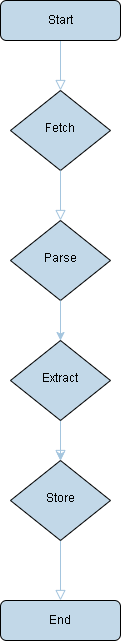
\includegraphics[height=15cm]{Figures/Web Scraper FlowChart.png} % Adjust the height here
    \caption{Web Scraper Flow Chart}
    \label{fig:enter-label}
\end{figure}


\begin{figure}
    \centering
    \includegraphics[width=1\linewidth]{Figures/UML.png}
    \caption{High level Overview}
    \label{fig:enter-label}
\end{figure}

\begin{figure}
    \centering
    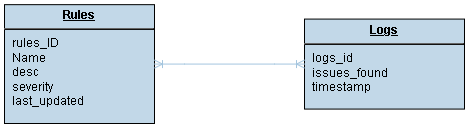
\includegraphics[width=1\linewidth]{Figures/database.drawio.png}
    \caption{Database Schema}
    \label{fig:enter-label}
\end{figure}
\begin{figure}
    \centering
    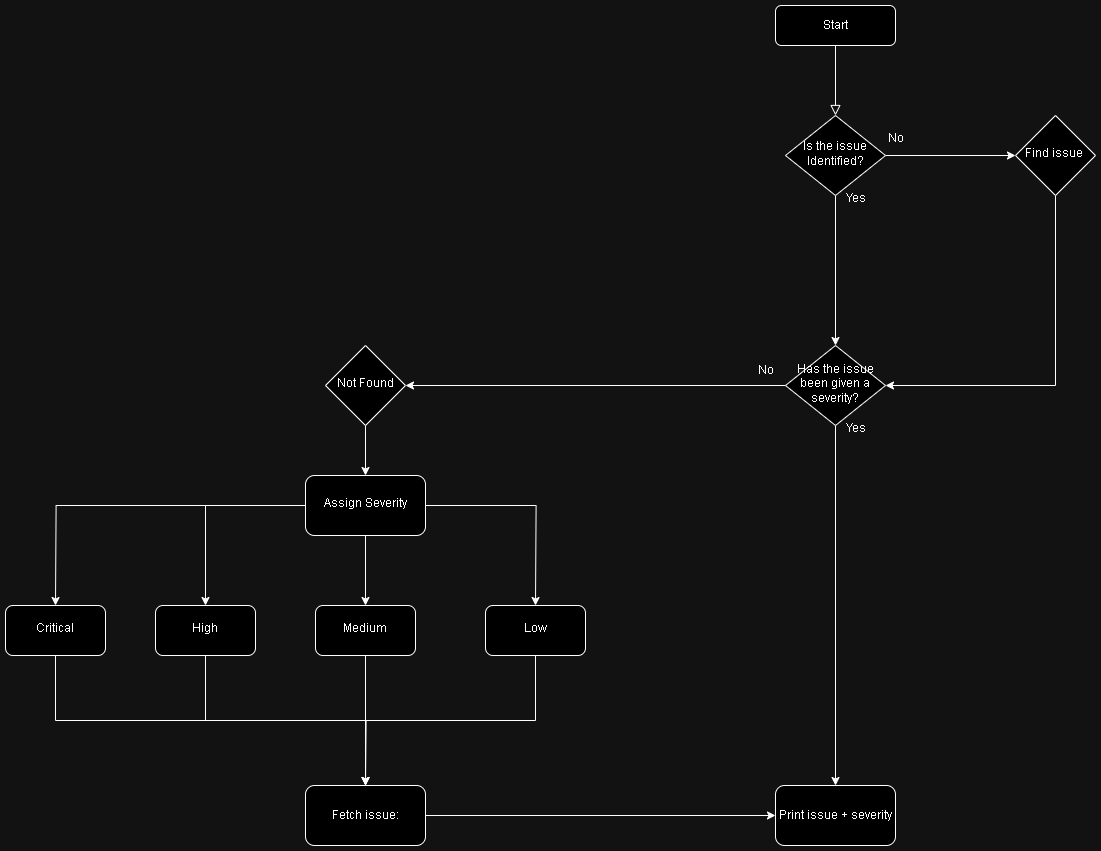
\includegraphics[width=1\linewidth]{Figures/prioritisation.drawio.png}
    \caption{Prioritisation Flow Chart}
    \label{fig:enter-label}
\end{figure} % Implementation Approach
\ifnum \value{semester}=1
\chapter{Conclusions and Future Work}
\label{chap:conclusions}
\lhead{\emph{Conclusions}}

\section{Discussion}
Reflecting on the research and development conducted during Semester 1, several challenges were encountered. Key issues included:
\begin{itemize}
    \item \textbf{Scope of Docker Smells}: Identifying and categorizing "Docker smells" was challenging due to the lack of a comprehensive, standardized dataset. The reliance on prior studies helped, but gaps in empirical coverage were evident.
    \item \textbf{Dynamic Rule Updates}: Integrating a reliable web-scraping mechanism posed technical challenges, especially in parsing ever-changing HTML structures from official documentation sites like Docker's. This led to considerations of fallback mechanisms for rule updates.
    \item \textbf{Performance vs. Real-Time Feedback}: Providing real-time linting feedback required optimization of the linting algorithms to balance thoroughness with responsiveness, especially in IDE environments.
    \item \textbf{CI/CD Pipeline Integration}: Ensuring compatibility across diverse CI/CD platforms (e.g., Jenkins, GitHub Actions) required modularity in the tool's architecture, adding complexity to the implementation plan.
\end{itemize}

These challenges informed key design decisions, such as leveraging SQLite for lightweight storage, prioritizing IDE integration for developer usability, and focusing on rule severity ranking for effective feedback. These learnings will guide the iterative improvements and expansions in Semester 2.

\section{Conclusion}
The Semester 1 phase established a solid foundation for the automated Docker linter. Significant conclusions include:
\begin{enumerate}
    \item \textbf{Importance of Smell Detection}: Docker smells like unpinned dependencies and excessive layering are pervasive and impactful, necessitating a robust detection mechanism.
    \item \textbf{Gap in Existing Tools}: Existing tools like Hadolint and Snyk address parts of the Docker quality landscape but lack comprehensive Docker smell detection with dynamic updates.
    \item \textbf{Shift-Left Security Impact}: By automating Dockerfile quality checks during development, this tool contributes significantly to early defect detection, improving developer workflows and CI/CD efficiency.
    \item \textbf{Architectural Feasibility}: A combination of Python for back-end processing, JavaScript for IDE extensions, and SQLite for rule storage offers a scalable and efficient architecture for the linter.
\end{enumerate}

These findings validate the problem statement and objectives defined earlier in the project, underscoring the necessity of this tool for modern containerized development workflows.

\section{Future Work}
Looking beyond Semester 1, several enhancements and expansions could significantly improve the Docker linter:
\begin{itemize}
    \item \textbf{Advanced AI Integration}:
    \begin{itemize}
        \item Explore machine learning models to predict and categorize new Docker smells dynamically, using large datasets of Dockerfiles from public repositories.
    \end{itemize}
    \item \textbf{Enhanced Rule Management}:
    \begin{itemize}
        \item Implement a robust conflict resolution mechanism for dynamically scraped rules to prevent inconsistencies across sources.
    \end{itemize}
    \item \textbf{Expanded IDE Support}:
    \begin{itemize}
        \item Extend integration to additional IDEs (e.g., JetBrains IntelliJ, Eclipse) to broaden the user base.
    \end{itemize}
    \item \textbf{Broader CI/CD Integration}:
    \begin{itemize}
        \item Add support for emerging CI/CD platforms and container orchestration tools like GitLab CI/CD and Kubernetes.
    \end{itemize}
    \item \textbf{Usability Studies}:
    \begin{itemize}
        \item Conduct developer feedback sessions to refine the tool's usability, focusing on intuitive UI/UX design for the IDE plug-in and quality reports.
    \end{itemize}
    \item \textbf{Open-Source Collaboration}:
    \begin{itemize}
        \item Open-source the project to foster community contributions, accelerating feature enhancements and establishing the tool as a widely adopted solution.
    \end{itemize}
    \item \textbf{Vulnerability Analysis Add-On}:
    \begin{itemize}
        \item Although excluded initially, a modular add-on for vulnerability scanning could complement the core functionality, making the tool more comprehensive.
    \end{itemize}
\end{itemize}

These avenues will ensure the linter continues evolving into a state-of-the-art tool for Dockerfile quality and security.

 % Semester 1 conclusion
\else
\chapter{Implementation}
\label{chap:imp}
\lhead{\emph{Project Implementation}}
This chapter details the development process of the Docker Linter Project, transitioning from the planned approach outlined in Chapter 4 to the final implemented solution. It documents the practical challenges encountered during the implementation phase (January - April), categorizes their severity, and analyzes their impact on the project's design, schedule, and outcomes. Furthermore, it provides an "as-built" specification by comparing the original plan (architecture, use cases, risks, methodology, schedule, evaluation, prototype) with the final developed project, justifying deviations based on the encountered difficulties.
\begin{itemize}
    \item \textbf{Easy:} The Challenge was easily resolved
    \item \textbf{Medium:} A significant challenge that required thought, research and problem solving to resolve
    \item \textbf{Hard:} Otherwise known as a blocker, a challenge that was too complex to resolve
and caused changes to the project’s functional and/or non-functional requirements
\end{itemize}
\section{Difficulties Encountered}
\label{sec:difficulties}
The development phase involved several technical and logistical challenges. These are categorized below based on their complexity and impact on the project's progression.

% --- Difficulty 1: LLM for Regex Generation ---
\subsection{Automating Rule Generation (English to Regex) using LLMs}
\label{subsec:llm_regex_difficulty} % Added label for potential cross-referencing
\begin{itemize}
    \item \textbf{Classification:} Hard
    \item \textbf{Description:} A significant challenge arose when attempting to automate the conversion of Docker best practices, often described in natural English, into precise regular expressions (Regex) suitable for the linter's rule engine. The goal was to leverage Large Language Models (LLMs) like gpt-4o to parse best practice descriptions (e.g., from docker official documentation ) and automatically generate corresponding Regex patterns. Despite experimenting with multiple LLMs and refining prompts to provide clear instructions and examples, the results were consistently unsatisfactory. The generated Regex patterns suffered from:
        \begin{itemize}
            \item \textbf{Inaccuracy:} Patterns often failed to correctly capture the understanding of the best practice, leading to potential false positives or false negatives during linting.
            \item \textbf{Inconsistency:} Even with the same input, the models produced varying outputs, making it impossible to generate reliable rules.
            \item \textbf{Over-simplification or Over-complexity:} Patterns were sometimes too general, matching unintended lines, or overly complex and inefficient.
        \end{itemize}
    \item \textbf{Impact on Original Project Design:}
        \begin{enumerate}
            \item \textbf{Architecture:} This directly impacted the planned mechanism for rule creation and updates. The failure of LLM automation necessitated a fallback to manual or semi-automated methods, affecting the architecture of the rule management component (potentially requiring more robust manual entry/validation interfaces or processes than initially envisioned if automation was heavily relied upon). It also impacted the envisioned workflow for updating rules based on newly scraped best practices.
            \item \textbf{Risk:} This represented an unforeseen technical risk not explicitly detailed in the initial assessment (Chapter 4, Section 4.2). While "Rule Conflicts" (Risk 6) and "Outdated Scraped Rules" (Risk 5) were identified, the difficulty of translating potentially valid scraped information into usable rules was underestimated. The failure introduced a risk of lower rule coverage or accuracy if manual generation couldn't keep pace or achieve the desired precision.
            \item \textbf{Methodology:} The Agile approach allowed for adapting to this challenge. Time initially allocated to LLM experimentation and integration within sprints had to be reallocated to manual rule creation and testing, demonstrating the methodology's flexibility.
            \item \textbf{Schedule:} Significant time was invested in exploring the LLM approach during the initial implementation phase (January-February). When this proved unsuccessful, it caused delays in populating the rule database,impacting subsequent tasks like comprehensive testing and IDE integration refinement which relied on a robust rule set. The schedule needed adjustment to accommodate the increased effort for manual rule generation.
            \item \textbf{Evaluation Plan:} The failure to automate rule generation meant relying on manual creation. This could impact the evaluation of smell detection (precision/recall) if the resulting rule set was less comprehensive than initially planned.
        \end{enumerate}
\item \textbf{Management Strategy:} The approach of using LLMs to automatically generate Regex rules from English descriptions proved unreliable, producing inaccurate and inconsistent patterns. Consequently, this automation attempt was abandoned. The strategy shifted entirely to manual Regex rule creation, which involved:
    \begin{itemize}
        \item Analyzing best practice descriptions from reliable sources (like Docker documentation).
        \item Manually writing and testing Regex patterns against sample Dockerfile lines making the Database redundant. 
        \item Storing these validated rules in a structured format (e.g., JSON/YAML in \texttt{Rules/}) with necessary metadata (severity, description, suggestion), drawing from structures like \texttt{Rules.json}.
    \end{itemize}
    These carefully crafted manual rules provided a reliable foundation for the linter's analysis engine (including any AI-driven components that used these rules), ensuring accuracy. However, this came at the cost of slower development and potentially fewer rules than planned with automation.
\end{itemize}

% --- Difficulty 2: Web Scraper Reliability --- (Based on Risk 10)
\subsection{Web Scraper Reliability and Maintenance}
\label{subsec:scraper_difficulty}
\begin{itemize}
    \item \textbf{Classification:} Medium
    \item \textbf{Description:} The web scraper (\texttt{webscraper.py}), originally designed to fetch Docker best practices from online sources to populate a dynamic rule database (as planned in Chapter 4, Section 4.1.2), faced intermittent failures. Websites frequently change their structure (HTML layout, CSS selectors), breaking the parsing logic. Ensuring the scraper consistently fetched information required ongoing monitoring and adjustments. This aligns with the anticipated “Web scraper failure” risk (Risk 10).  
    \newline\textit{Note: Even though rule generation is now manual, the GPT-4o analysis engine still loads the scraper’s JSON output at runtime to stay informed of any newly scraped best practices.}

    \item \textbf{Impact on Original Project Design:}
        \begin{enumerate}
            \item \textbf{Architecture:} The failure of LLM-based rule generation (Section \ref{subsec:llm_regex_difficulty}) reduced the scraper’s role in directly feeding the linter’s active rule set. It now primarily serves as a discovery tool—its JSON output is consumed by GPT-4o for AI-driven analysis rather than auto-populating the database.
            \item \textbf{Risk:} Realized the high‐frequency “Web scraper failure” risk (Risk 10). Its reduced direct impact on rules did not eliminate the maintenance effort.
            \item \textbf{Methodology:} Sprints allocated time for scraper upkeep, though at lower priority given its secondary role.
            \item \textbf{Schedule:} Introduced minor, unpredictable delays for scraping fixes, with less effect on core linting development than originally anticipated.
            \item \textbf{Evaluation Plan:} Since dynamic rule updates via scraping are no longer automatic, evaluation of “Outdated Scraped Rules” shifted focus to manual review of discovered practices.
        \end{enumerate}

    \item \textbf{Management Strategy:} Even with its reduced role, we kept the scraper reliable as a discovery source and AI input:
        \begin{itemize}
            \item \textbf{Robust Error Handling:} Wrapped network calls and HTML parsing in \texttt{try-except} to catch connection or DOM‐change errors, preventing crashes.
            \item \textbf{Detailed Logging:} Used Python’s \texttt{logging} to record URLs, timestamps, success/failure status, and exceptions for quick diagnosis.
            \item \textbf{Simplified Validation:} Periodically ran the scraper against key sources to confirm basic functionality and data extraction.
            \item \textbf{Source Prioritization:} Focused on the most stable, authoritative sites (e.g., Docker docs) rather than broad diversification.
            \item \textbf{AI Integration:} Ensured GPT-4o reads the scraper’s JSON each run to refresh its knowledge of best practices—keeping AI analysis aligned with scraped sources even though rule enforcement is manual.
            \item \textbf{Reactive Maintenance:} Treated breakages as bugs, fixing selectors or parsing logic as part of routine sprint backlog grooming.
        \end{itemize}
\end{itemize}

% --- Difficulty 3: Dockerfile Optimization & Linter Application --- (Based on explanation.txt)
\subsection{Implementing Dockerfile Optimizations}
\label{subsec:optimization_difficulty}
\begin{itemize}
    \item \textbf{Classification:} Medium
    \item \textbf{Description:} Applying linter recommendations (multi-stage builds, non-root users, combining \texttt{RUN} steps, using \texttt{COPY} instead of \texttt{ADD}, pinning versions) to our own Dockerfile required careful testing to avoid build or runtime breakages.
    \item \textbf{Impact on Original Project Design:}
        \begin{enumerate}
            \item \textbf{Architecture:} Produced a more complex, multi-stage Dockerfile, improving deployment structure.
            \item \textbf{Risk:} Raised security and efficiency but occasionally triggered new build failures.
            \item \textbf{Methodology:} Used Agile's iterative cycles to implement and verify each change.
            \item \textbf{Schedule:} Allocated extra time for rebuilding and debugging after each optimization.
            \item \textbf{Evaluation Plan:} Showed image size reductions and faster builds, satisfying the "Optimising Performance" goal.
        \end{enumerate}
    \item \textbf{Management Strategy:} The project's own Dockerfile optimizations were applied and tested in a single workflow rather than step-by-step rebuilds:
        \begin{itemize}
            \item \textbf{AI-Driven Rewrite:} Generated a complete optimized Dockerfile via GPT-4o, incorporating linter findings and best practices.
            \item \textbf{Post-Processing:} Cleaned the AI output (e.g., removed incompatible version pins) to ensure compatibility with the chosen base image.
            \item \textbf{Single Build Verification:} Built the optimized image once to collect size and layer metrics.
            \item \textbf{Version Control:} Committed the final, verified Dockerfile with clear messages and used Git's rollback on any post-merge issues.
            \item \textbf{Documentation:} Added inline comments in the Dockerfile and descriptive commit notes explaining each major change and its benefit.
        \end{itemize}
\end{itemize}

% --- Difficulty 4: Integration Complexity (VS Code / Jenkins) ---
\subsection{Integration Complexity (VS Code / Jenkins)}
\label{subsec:integration_difficulty}
\begin{itemize}
  \item \textbf{Classification:} Medium
  \item \textbf{Description:} Integrating the linter with VS Code (\texttt{VS-Extension}) required understanding the VS Code API for diagnostics and commands. Similarly, setting up Jenkins pipelines (\texttt{jenkins}) to execute the linter (e.g.\ \texttt{lint\_cli.py}) involved configuring build steps, handling outputs, and managing execution environments. Specific API calls and pipeline syntax often needed troubleshooting and experimentation.
  \item \textbf{Impact on Original Project Design:} Primarily affected the schedule, requiring dedicated time for understanding external tool APIs and configurations. This directly tests the planned mitigation for Risk 1 (CI/CD integration testing).
  \item \textbf{Management Strategy:} Addressed external-tool complexities through focused research and iterative testing:
    \begin{itemize}
      \item \textbf{Targeted Documentation Review:} Consulted VS Code’s \texttt{DiagnosticCollection} and \texttt{commands} API docs, and Jenkins Pipeline syntax for \texttt{sh} steps, exit-code handling, and report plugins (e.g.\ Warnings NG).
      \item \textbf{Example-Driven Development:} Adapted community examples (Stack Overflow, official tutorials) to bootstrap extension and pipeline scripts.
      \item \textbf{Incremental Testing and Debugging:}
        \begin{itemize}
          \item \textbf{VS Code:} Verified the extension loads; tested lint on save/open; parsed JSON output from \texttt{lint\_cli.py} into diagnostics; added custom commands (e.g.\ ignore rule).
          \item \textbf{Jenkins:} 
            \begin{enumerate}
              \item Checkout code.
              \item Execute \texttt{sh 'python lint\_cli.py --format json || exit 1'} to fail on non-zero exit.
              \item Verify output in console logs.
              \item Put output into Jenkins artifacts ( like .csv files)
            \end{enumerate}
        \end{itemize}
    \end{itemize}
\end{itemize}
% --- Difficulty 5: Lack of Benchmark Datasets ---
\subsection{Lack of Public Benchmark Datasets for Evaluation}
\label{subsec:benchmark_difficulty}
\begin{itemize}
    \item \textbf{Classification:} Medium
    \item \textbf{Description:} A significant hurdle was encountered during the evaluation phase (Chapter 6) when attempting to find publicly available, standardized datasets of Dockerfiles with known, labeled vulnerabilities or "smells" (anti-patterns). While general code vulnerability datasets exist, datasets specifically curated for Dockerfile best practices and common security flaws targeted by this linter were scarce or non-existent. Existing Dockerfile collections often lacked ground-truth annotations regarding adherence to specific best practices (like those enforced by the linter's rules), making objective measurement of the linter's precision and recall difficult using external benchmarks.
    \item \textbf{Impact on Original Project Design:}
        \begin{enumerate}
            \item \textbf{Evaluation Plan:} This directly impacted the planned methodology for evaluating the linter's effectiveness (precision/recall metrics). The inability to use established benchmarks necessitated a pivot to creating a custom benchmark dataset, requiring additional time and effort not initially budgeted within the evaluation phase. It also meant the evaluation results would be based on this custom benchmark, potentially limiting direct comparability with other tools evaluated on different (hypothetical) datasets.
            \item \textbf{Risk:} Introduced the risk that the custom-created benchmark might not be fully representative of real-world Dockerfiles or could unintentionally favour the linter's specific rule set, potentially biasing the evaluation results.
            \item \textbf{Schedule:} Substantial time had to be allocated within the evaluation period (or potentially extending it) to curate, analyze, and label Dockerfiles for the custom benchmark.
        \end{enumerate}
    \item \textbf{Management Strategy:}
        \begin{itemize}
            \item \textbf{Custom Benchmark Creation:} Since no suitable public dataset was found, a custom benchmark dataset was manually created. This involved:
                \begin{itemize}
                    \item Collecting a diverse set of Dockerfiles from various sources (e.g., GitHub repositories, public examples, potentially anonymized internal projects) to ensure variety in complexity, base images, and application types.
                    \item Manually analyzing each Dockerfile against the linter's defined rule set (\texttt{Rules/}).
                    \item Carefully labeling each Dockerfile (or specific lines within them) with the ground truth – identifying which rules should be triggered (true positives) and which parts were compliant (true negatives).
                    \item Documenting the benchmark creation process and the criteria used for labeling to ensure transparency and potential reproducibility.
                \end{itemize}
            \item \textbf{Targeted Evaluation:} The evaluation metrics (precision, recall, F1-score) were then calculated based on the linter's performance against this custom-built, manually-labeled dataset.
            \item \textbf{Acknowledging Limitations:} The evaluation results explicitly noted that they were based on a custom benchmark due to the lack of public alternatives, acknowledging the potential limitations this entails.
        \end{itemize}
\end{itemize}

% --- Difficulty 6: AI Analysis Latency and Cost ---
\subsection{AI Analysis Latency and Cost}
\label{subsec:ai_latency_cost_difficulty}
\begin{itemize}
    \item \textbf{Classification:} Medium
    \item \textbf{Description:} Integrating GPT-4o for Dockerfile analysis, while powerful, introduced challenges related to API call latency and cost. Real-time analysis, especially within the VS Code extension (\texttt{VS-Extension}), could feel sluggish due to the time required for the API roundtrip. Furthermore, frequent analysis (e.g., on every file save) could lead to accumulating API costs that needed monitoring and management. Balancing the benefit of AI insights with performance and budget was key. \textit{Note: This is distinct from the LLM's failure for regex generation (Section \ref{subsec:llm_regex_difficulty}) and focuses on the operational aspects of using the AI for analysis.}
    \item \textbf{Impact on Original Project Design:}
        \begin{enumerate}
            \item \textbf{Architecture:} May have required implementing asynchronous processing for AI calls in the \texttt{VS-Extension} to avoid blocking the UI. Caching mechanisms might have been considered to avoid redundant API calls for unchanged file parts.
            \item \textbf{Risk:} Potential for poor user experience due to latency (Risk 9: Performance Issues, but specific to AI). Risk of exceeding budget if API usage wasn't controlled.
            \item \textbf{Methodology/Schedule:} Required adjustments to optimize prompt design for speed and potentially adding configuration options for users to control AI analysis frequency or disable it.
        \end{enumerate}
    \item \textbf{Management Strategy:}
        \begin{itemize}
            \item \textbf{Asynchronous Execution:} Implemented non-blocking API calls in the VS Code extension so the UI remained responsive during AI analysis.
            \item \textbf{Prompt Optimization:} Refined prompts sent to GPT-4o to be more concise and focused, potentially reducing processing time and token usage.
        \end{itemize}
\end{itemize}

% --- Difficulty 7: Defining and Maintaining Rule Quality ---
\subsection{Defining and Maintaining Rule Quality}
\label{subsec:rule_quality_difficulty}
\begin{itemize}
    \item \textbf{Classification:} Medium
    \item \textbf{Description:} Following the shift to manual rule creation (Section \ref{subsec:llm_regex_difficulty}), ensuring the \textit{quality} and \textit{maintainability} of the rule set in \texttt{Rules/} became a significant, ongoing task. This involved not just writing Regex, but also crafting clear, unambiguous rule descriptions, providing genuinely helpful suggestions for remediation, assigning appropriate severity levels, and rigorously testing each rule against a diverse set of Dockerfiles to minimize both false positives and false negatives. Establishing a consistent standard and process for rule lifecycle management (creation, testing, updates, deprecation) was crucial but time-consuming.
    \item \textbf{Impact on Original Project Design:}
        \begin{enumerate}
            \item \textbf{Architecture:} Led to a more structured format for rule definitions (e.g., the \texttt{Rules.json} structure) incorporating metadata beyond just the regex (description, suggestion, severity, perhaps links to documentation). Required building a robust testing framework specifically for rules.
            \item \textbf{Risk:} Poorly defined or tested rules could lead to user frustration (irrelevant warnings, missed issues) and undermine the linter's credibility. Directly impacts the effectiveness measure in the \texttt{Evaluation Plan}.
            \item \textbf{Schedule:} Allocated significant, continuous effort throughout the project lifecycle for rule refinement and testing, beyond the initial creation phase.
        \end{enumerate}
    \item \textbf{Management Strategy:}
        \begin{itemize}
            \item \textbf{Standardized Rule Schema:} Defined and enforced a clear JSON/YAML schema for rules in \texttt{Rules/}, including mandatory fields for ID, severity, description, suggestion, and the regex pattern.
            \item \textbf{Rule Validation Test Suite:} Created a dedicated suite of test Dockerfiles containing examples that should trigger specific rules and examples that should \textit{not}, allowing for automated testing of rule accuracy (precision/recall).
            \item \textbf{Peer Review Process:} Implemented a review process for any new or modified rules before merging them into the main rule set.
            \item \textbf{Documentation Links:} Where applicable, included links to official documentation or best practice guides within rule descriptions/suggestions.
            \item \textbf{Regular Review Cycle:} Periodically reviewed the existing rule set for relevance and accuracy against the latest Docker best practices.
        \end{itemize}
\end{itemize}
\section{Actual Solution Implementation}
\label{sec:actual_solution}

The solution implemented between January and April evolved significantly from the initial design outlined in \refchapfour{}. This evolution was primarily driven by the technical challenges encountered (\refsecdifficulties{}) and the practicalities of development. This section contrasts the initial plan with the final delivered architecture and components.

\subsection{Initial Design (as planned in \ref{sec:Arch})}
\begin{figure}[h!]
    \centering
    \includegraphics[width=1\linewidth]{Figures/UML.png} % Adjusted width slightly
    \caption{Original Overview of the Implemented Architecture}
    \label{fig:original_architecture} % Changed label for clarity
\end{figure}
The originally envisioned architecture centred around several key components:
\begin{itemize}
    \item A Python backend, likely using Flask, to serve as an API endpoint.
    \item An LLM-based system for automatically generating Regex rules from natural language descriptions of Docker best practices.
    \item A web scraping component (\texttt{BeautifulSoup}) to gather best practices from online sources.
    \item A database (planned as SQLite) to store the generated rules.
    \item A VS Code extension (JavaScript) for IDE integration.
    \item Jenkins integration for CI/CD pipeline checks.
\end{itemize}
This design heavily relied on the successful automation of rule generation via LLMs. (Refer to \refchapfour{} for the detailed initial plan).

\subsection{Final Implemented Architecture}
The architecture implemented by the project deadline is depicted in Figure \ref{fig:final_architecture}.
\begin{figure}[H] % Use [h!] to suggest placing it here if possible
    \centering
    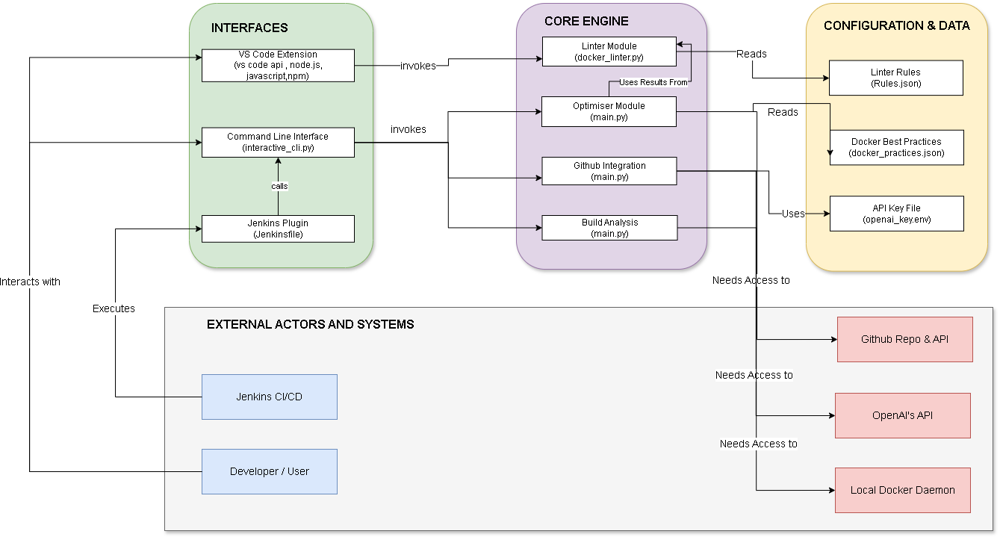
\includegraphics[width=1\linewidth]{Figures/FinalUML.png} % Adjusted width slightly
    \caption{Final Implemented Architecture Overview}
    \label{fig:final_architecture} % Changed label for clarity
\end{figure}

The final system consists of the following core components:
\begin{itemize}
    \item \textbf{Interfaces:} Provides points of interaction for users and external systems.
        \begin{itemize}
            \item \textbf{VS Code Extension (\texttt{VS-Extension}):} Developed using JavaScript/Node.js and the VS Code API to provide real-time linting feedback within the IDE. Invokes the Core Engine.
            \item \textbf{Command Line Interface (\texttt{interactive\_cli.py}):} A Python script allowing direct user interaction and testing. Invokes the Core Engine.
            \item \textbf{Jenkins Plugin (\texttt{Jenkinsfile}):} Enables integration into CI/CD pipelines.
        \end{itemize}

    \item \textbf{Core Engine (Python):} Handles the primary logic of linting, analysis, and integration.
        \begin{itemize}
            \item \textbf{Linter Module (\texttt{dockerfile\_linter.py}):} Performs the fundamental Dockerfile analysis based on the defined rules. Reads from Configuration \& Data.
            \item \textbf{Supporting Modules (\texttt{main.py}):} While shown as separate conceptual blocks in the diagram (Optimiser, GitHub Integration, Build Analysis), these functionalities are implemented within \texttt{main.py}. This includes coordinating analysis,suggesting optimizations (using Linter results), interacting with GitHub APIs, and analysing build information. Reads from and Uses Configuration \& Data. Needs access to External Systems (GitHub API, OpenAI API, Docker Daemon).
        \end{itemize}

    \item \textbf{Configuration \& Data:} Stores the rules, knowledge, and settings used by the Core Engine.
        \begin{itemize}
            \item \textbf{Linter Rules (\texttt{Rules/Rules.json}):} Contains the manually created and validated rule set (Regex patterns, descriptions, suggestions) following the abandonment of LLM-based generation. Read by the Linter Module.
            \item \textbf{Docker Best Practices (\texttt{docker\_practices.json}):} Likely stores structured information gathered by the web scraper (\texttt{webscraper.py}), serving as a knowledge base for AI analysis components or informing manual rule updates. Read by the Core Engine. The scraper itself required ongoing maintenance (\refsubsecreliability{}).
            \item \textbf{API Key File (\texttt{openai\_key.env}):} Stores necessary credentials for accessing external APIs (e.g., OpenAI). Used by the Core Engine.
        \end{itemize}

    \item \textbf{External Actors and Systems (Dependencies):} While not internal components, the system relies on:
        \begin{itemize}
            \item \textbf{Developer/User:} Interacts via VS Code or CLI.
            \item \textbf{Jenkins CI/CD:} Executes the linter via the Jenkins Plugin/CLI.
            \item \textbf{GitHub Repo \& API:} Accessed by the Core Engine for integration features.
            \item \textbf{OpenAI's API:} Accessed by the Core Engine for AI-driven analysis features.
            \item \textbf{Local Docker Daemon:} Accessed by the Core Engine for build analysis or related tasks.
        \end{itemize}
\end{itemize}

\subsection{Comparison and Justification of Changes}

Comparing the initial plan to the final implementation reveals key deviations driven by necessity and practicality:

\begin{itemize}
    \item \textbf{Rule Generation and Storage:} Since using LLMs to automatically generate Regex proved unreliable, we shifted to a fully manual process for creating, checking, and storing rules. We use flat files (Rules) for storage because they are simple and easy to version control. This improved rule quality but slowed development and potentially reduced the number of rules compared to our original automated approach
    \item \textbf{API vs. CLI/IDE Focus:} The planned Flask API was not implemented. Focus shifted to the command-line interfaces  (\texttt{interactive\_cli.py}) and the VS Code extension as the primary methods for users and systems (like Jenkins) to interact with the linter. This provided more direct value for the core developer and CI/CD use cases within the project timeframe, especially given the resources redirected to manual rule creation and scraper maintenance (\refsubsecreliability{}).
    \item \textbf{Use Case Scope:} While the core use cases (CLI linting, IDE feedback, CI/CD checks) were successfully implemented, the scope of "smell detection" was directly tied to the number and quality of manually created rules. The LLM failure (\refsubsecllmregex{}) meant the project couldn't achieve the breadth of automated rule coverage initially hoped for. The "real-time" aspect in the IDE was implemented, but potential latency from external calls (e.g., Python script execution, potential AI analysis calls) needed consideration (\refsubseclatency{}).
    \item \textbf{Risk Realization and Management:} Several planned risks materialized. Web scraper fragility (Risk 10) required ongoing maintenance (\refsubsecreliability{}). CI/CD and IDE integration complexities (Risk 1, Risk 11) were addressed during implementation (\refsubsecintegration{}). An unforeseen major risk emerged regarding the difficulty of translating requirements into reliable rules, especially via LLMs (\refsubsecllmregex{}). The lack of suitable benchmark datasets (\refsubsecbenchmark{}) also presented a challenge during evaluation. Optimizations were applied to the project's own Dockerfile (\refsubsecoptimization{}), potentially mitigating performance risks (Risk 9) for that specific case, though general performance might still be a factor depending on file size and rule complexity.
\end{itemize}

\subsection{(iii) Risk Assessment}
Original Plan: Identified risks including scraper failure, rule conflicts, performance, CI/CD integration issues (Table \ref{tab:ProjRisks}).

Actual Implementation:
\begin{itemize}
    \item The "Web scraper failure" risk (Risk 10) materialized and required ongoing management (Section \ref{subsec:scraper_difficulty}). Mitigation strategies (error handling, monitoring) were crucial.
    \item An unforeseen risk related to the difficulty of translating best practices into rules (especially via automation) emerged and proved significant (Section \ref{subsec:llm_regex_difficulty}).
    \item Risks related to CI/CD or IDE integration (Risk 1, Risk 11) were likely managed during implementation.
\end{itemize}
Deviation: The risk profile shifted, with the rule generation process proving more challenging than initially anticipated.

Justification: Implementation revealed the practical complexities behind some risks (scraper fragility) and uncovered new ones (LLM limitations).

\subsection{(iv) Methodology}
Original Plan: Agile-Scrum methodology.

Actual Implementation: The Agile-Scrum approach appears to have been followed.

Deviation: None explicitly noted, but the methodology's flexibility was likely tested.

Justification: The ability to adapt sprints based on unforeseen challenges like the LLM automation failure (Section \ref{subsec:llm_regex_difficulty}) and scraper maintenance (Section \ref{subsec:scraper_difficulty}) demonstrates the value of the chosen Agile approach. Resources were reallocated from the failing LLM path to manual rule creation.

\subsection{(v) Implementation Schedule}
Original Plan: Detailed Jan-June schedule (Chapter 4, Section 4.4). Jan: Setup, Enhance Prototype; Feb: IDE/DB Integration; Mar: CI/CD, Optimization; Apr: Testing, Reports.

Actual Implementation:
\begin{itemize}
    \item Setup, core linter development, web scraping likely occurred in Jan/Feb.
    \item IDE and CI/CD integration work likely followed.
\end{itemize}
Deviation: The schedule likely experienced delays, particularly in rule set completion and potentially advanced feature testing, due to the time spent on the unsuccessful LLM automation attempt (Section \ref{subsec:llm_regex_difficulty}) and ongoing scraper maintenance (Section \ref{subsec:scraper_difficulty}). Tasks planned for Feb/March might have shifted into March/April. Optimization work (Section \ref{subsec:optimization_difficulty}) also required dedicated time.

Justification: Unforeseen technical hurdles (LLM failure) and the practical demands of maintaining components like the web scraper necessitated schedule adjustments. Prioritization shifted towards ensuring core functionality with manually curated rules.

\subsection{(vi) Evaluation Plan}
Original Plan: Comprehensive plan with quantitative and qualitative metrics, controlled experiments, and real-world testing (Chapter 4, Section 4.5).

Actual Implementation:
\begin{itemize}
    \item The groundwork for evaluation (e.g., linter CLI for testing, potential test cases in `testing/`) was likely laid.
\end{itemize}
Deviation: The scope of the evaluation might have been adjusted based on the final state of the rule set and features. For instance, comparisons against Hadolint/Snyk might focus on a core set of implemented rules due to the manual bottleneck caused by the LLM failure (Section \ref{subsec:llm_regex_difficulty}). Measuring precision/recall might be based on this implemented rule set. Collection of all planned metrics (e.g., latency, developer surveys) might depend on the final implementation status by the end of April.

Justification: The evaluation plan needed to reflect the achievable scope of the project by the deadline, potentially prioritizing validation of the core, manually implemented rules and key integrations over broader comparisons or metrics impacted by the rule generation difficulties.

\subsection{(vii) Prototype}
Original Plan: Included flow charts (Web Scraper, Prioritization), UML diagram, DB schema (Chapter 4, Section 4.6).

Actual Implementation:
\begin{itemize}
    \item The final architecture likely aligns broadly with the UML diagram, showing components like the linter engine, rule storage, scraper, and integrations.
    \item The database schema (`DB/`) might closely follow the prototype, adjusted for manual rule storage.
    \item The web scraper flow likely follows the chart, incorporating the necessary error handling identified as crucial (Section \ref{subsec:scraper_difficulty}).
\end{itemize}
Deviation: The exact implementation details might differ slightly from the initial diagrams based on libraries chosen or refinements made during coding. The rule prioritization logic might have been simplified if the rule set itself was smaller than anticipated post-LLM failure.

Justification: Prototypes serve as a starting point; minor deviations during implementation are normal as technical details are finalized. The core concepts from the prototype likely guided the development. % Actual Implementation
\chapter{Testing and Evaluation}
\label{chap:eval}
\lhead{\emph{Project Testing}}
The goal of this chapter is an objective evaluation of the final AI Docker Linter \& Optimizer system. The evaluation focuses on quantitative metrics to assess the system's effectiveness, accuracy, and performance. Where applicable, a comparative analysis is performed against Hadolint, a widely used static analysis tool for Dockerfiles. The testing utilizes a benchmark dataset of Dockerfiles to evaluate the system's ability to achieve its core objectives in realistic scenarios.

\section{Metrics}
\label{sec:eval_metrics}
To evaluate the system comprehensively, the following key metrics were identified and measured:

\begin{itemize}
    \item \textbf{Optimization Effectiveness:}
        \begin{itemize}
            \item \textbf{Build Success Rate (\%):} The percentage of Dockerfiles from the test set for which the optimized version could be successfully built into a Docker image. This measures the reliability and correctness of the optimization component.
            \item \textbf{Average Image Size Reduction (\%):} For successfully optimized Dockerfiles built, the average percentage reduction in final image size compared to the original Dockerfile image size. This quantifies the primary goal of reducing image bloat.
        \end{itemize}
    \item \textbf{Linter Accuracy (Comparison with Hadolint):} To evaluate the AI-driven linter component, its ability to identify potential issues (violations of best practices) was compared with Hadolint using standard classification metrics.
        \begin{itemize}
            \item \textbf{Precision:} The proportion of issues identified (by the linter) that were actual issues (true positives) out of all problems identified by the linter (true positives + false positives). \( \text{Precision} = \frac{TP}{TP + FP} \)
            \item \textbf{Recall:} The proportion of actual issues that were correctly identified by the linter (true positives) out of all actual issues present (true positives + false negatives). \( \text{Recall} = \frac{TP}{TP + FN} \)
            \item \textbf{F1-Score:} The harmonic mean of Precision and Recall, providing a single measure of the linter's accuracy. \( \text{F1 Score} = 2 \times \frac{\text{Precision} \times \text{Recall}}{\text{Precision} + \text{Recall}} \)
        \end{itemize}
        These metrics were calculated for both the custom AI linter and Hadolint based on a manually annotated ground truth for the Dockerfile test set.
    \item \textbf{Performance:}
        \begin{itemize}
            \item \textbf{Average Analysis Duration (seconds):} The average time taken by the system to fully analyze and process a single Dockerfile (including linting and optimization suggestion).
            \item \textbf{Analysis Duration vs. Dockerfile Size:} Correlation between the analysis duration and the size (number of lines) of the input Dockerfile. This helps understand the scalability and performance characteristics of the tool.
        \end{itemize}
\end{itemize}

\section{System Testing}
\label{sec:eval_setup}
The evaluation was conducted using a defined experimental setup to ensure reproducible and objective measurements.

\begin{itemize}
    \item \textbf{Dataset:} A benchmark set of 7 Dockerfiles (\texttt{testing/Dockerfiles\_set/}) was used as input for the evaluation. This set was chosen to represent a variety of common use cases and complexities. [\emph{Optional: Add more detail here if you know the origin or specific characteristics of this dataset, e.g., "sourced from popular open-source projects" or "specifically crafted to test various Dockerfile instructions."}]
    \item \textbf{Experimental Process:}
        \begin{enumerate}
            \item Each Dockerfile in the dataset was processed by the AI Docker Linter \& Optimizer system.
            \item For optimization evaluation, the tool generated an optimized version of the Dockerfile. An attempt was made to build a Docker image from both the original and the optimized Dockerfile. Image sizes were recorded, and the build success/failure was noted.
            \item For linter evaluation, both the custom AI linter and Hadolint were run on the original Dockerfiles. Their outputs were compared against a pre-defined ground truth (manual annotation of actual issues) to calculate Precision, Recall, and F1-Score.
            \item The time taken for the AI system to analyze each Dockerfile was recorded.
            \item The number of lines in each Dockerfile was recorded to analyze correlation with processing time.
        \end{enumerate}
    \item \textbf{Tooling:} The experiments were automated using Python scripts. The primary script, \texttt{testing/evaluate\_results.py}, orchestrated the processing of Dockerfiles, interaction with the AI tool, execution of Hadolint, Docker image builds, and collection of raw data. The script \texttt{testing/generate\_graphs.py} was used subsequently to process the raw data (stored in \texttt{testing/evaluation\_summary.json}) and generate visualizations.
\end{itemize}

\section{Results}
\label{sec:eval_results}
The evaluation yielded quantitative results across the defined metrics, summarized below. The raw aggregated data can be found in \texttt{testing/evaluation\_summary.json}.
\begin{itemize}
    \item \textbf{Optimization Effectiveness (Issue Counts):} A comparison based on the number of issues resolved, unresolved, and newly introduced revealed the following:
        \begin{itemize}
            \item \textbf{Resolved Issues:} The Custom Method resolved 53 issues, while ChatGPT-4o resolved 52 issues. Both methods showed comparable effectiveness in resolving existing issues.
            \item \textbf{Unresolved Issues:} The Custom Method left 0 issues unresolved, while ChatGPT-4o left 1 issue unresolved.
            \item \textbf{New Issues Introduced:} The Custom Method introduced 9 new issues during optimization, significantly fewer than the 29 new issues introduced by ChatGPT-4o.
            \item Overall, while both methods were effective at resolving issues, the Custom Method introduced considerably fewer new problems.
        \end{itemize}
        Figure \ref{fig:opt_eff} illustrates this comparison.
         \begin{figure}[ht]
            \centering
            % Ensure the image path 'testing/optimization_comparison.png' exists
            % or update it to the correct path for Figure 6.1
            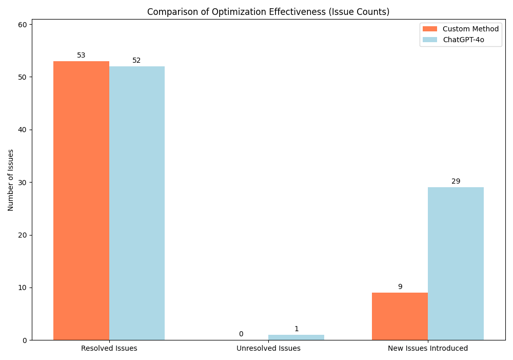
\includegraphics[width=0.8\textwidth]{Figures/Picture3_comparisonAI.png}
            \caption{Comparison of Optimization Effectiveness (Issue Counts): Custom Method vs. ChatGPT-4o.}
            \label{fig:opt_eff}
        \end{figure}

% The closing \end{itemize} should be present from the parent list structure
% \end{itemize}


     \item \textbf{Performance:}
        \begin{itemize}
            \item The \textbf{Average Analysis Duration} per Dockerfile was \textbf{64.80 seconds}. 
            \item One file analysis took significantly longer (303 seconds), which substantially skews this average. The median duration or an average calculated without this outlier might offer a more representative measure of typical performance.
            \item Figure \ref{fig:time_corr} illustrates the relationship between the analysis duration and the Dockerfile size (in lines). The plot shows variability in analysis time, particularly highlighting the outlier, and allows for visual assessment of any correlation between file size and processing time. % You can add specific observations here, e.g., "showing a weak positive correlation" or "indicating increased variance for larger files" once you interpret the graph.
        \end{itemize}
         \begin{figure}[ht]
            \centering
            % Ensure the path 'Figures/Picture3_size.png' is correct
            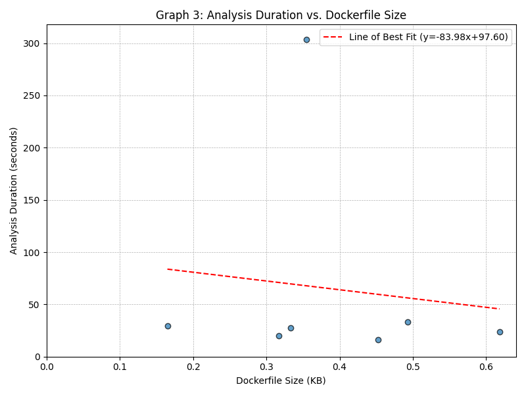
\includegraphics[width=0.8\textwidth]{Figures/Picture3_size.png} 
            \caption{Analysis Duration vs. Dockerfile Size (Lines).}
            \label{fig:time_corr}
        \end{figure}

\end{itemize}

\textbf{Threats to Validity:}
Potential threats to the validity of these results include:
\begin{itemize}
    \item \textbf{Dataset Size and Representativeness:} The evaluation used a limited set of 7 Dockerfiles. A larger, more diverse dataset might yield different average results or reveal edge cases not encountered.
    \item \textbf{Ground Truth Accuracy:} The linter accuracy metrics depend on the correctness and completeness of the manual annotation (ground truth) used for comparison. Any errors in annotation would affect the calculated Precision, Recall, and F1-Scores.
    \item \textbf{Build Environment Consistency:} Docker build processes can sometimes be affected by caching or network conditions, although efforts were made to ensure a consistent environment for comparing original and optimized builds.
    \item \textbf{Complexity of Analysis Task:} The performance metrics, particularly analysis time, are specific to the complexity of the tasks performed by this specific AI model and optimization logic. Different approaches might have different performance characteristics.
\end{itemize}
These factors should be considered when interpreting the results. A more detailed discussion follows in Chapter 5.
 % Testing
\chapter{Discussion and Conclusions}
\label{chap:conclusions}
\lhead{\emph{Discussion and Conclusions}}
In this chapter, you should expand upon (and initially reflect upon) the discussion and conclusion of the research phase of the project. The expectation here is that you should discuss the results presented in the previous evaluation section of the project in their totality (i.e. as a whole) from which you will then draw clear conclusions both on the quantitative and qualitative aspects of the overall project. This chapter should be a about 2000 words long (5 pages of text - 1600 words of discussion and 400 words of conclusion). This may vary depending on quality. The conclusion section of this report should conclude the project.

Some suggested sections (the nature of this chapter should be discussed in detail with your term 2 supervisor):

\section{Solution Review}
Discuss how well your solution solves the problem, based on your results from the evaluation chapter.

\section{Project Review}
Discuss how well you addressed the project, and what you might do differently if you were to do it again. Make sure to identify how you handled any problems that arose during the project. Identify key skills that you learnt during the project, and clearly describe how you applied these, and how you might apply them differently if you were to do a similar project.

\section{Conclusion}
Enumerate the main conclusions you have got in terms of background, problem description and the solution approach you have come up with. Detail your primary and any secondary conclusions from your project.

\section{Future Work}
Discuss any proposals for completion of the project, or for enhancements, or for re-design of your solution or software. Enumerate all the things you would have wanted to do should you have more time to work on this project. % Discussion and Conclusion
\fi

%% ----------------------------------------------------------------
\label{Bibliography}
\bibliographystyle{IEEEtranN}  % Use the "IEEE Transaction" BibTeX style for formatting the Bibliography
\bibliography{Information/Bibliography}  % The references (bibliography) information are stored in the file named "Bibliography.bib"
\lhead{\emph{Bibliography}}  % Change the left side page header to "Bibliography"

%% ----------------------------------------------------------------
% Now begin the Appendices, including them as separate files

\addtocontents{toc}{\vspace{2em}} % Add a gap in the Contents, for aesthetics

\appendix % Cue to tell LaTeX that the following 'chapters' are Appendices

\chapter{Code Snippets}

Put appendix material in this section e.g. code snippets 

USE THE APPENDICES	% Appendix A
\chapter{Wireframe Models} % Appendix B


\addtocontents{toc}{\vspace{2em}}  % Add a gap in the Contents, for aesthetics
\backmatter
\end{document}  % The End
%% ----------------------------------------------------------------
